\chapter{Experimental Data} \label{chap:experiment}
In order to validate the performance of the observer implementation, experimental data was collected with a Hokuyo UBG-04LX-F01 scanning laser range-finder.

Measurements were taken to:
\begin{itemize}
\item build a model of the noise characteristics of the Hokuyo UBG-04LX-F01 in order to more accurately simulate the performance of the observer;
\item observe the motion of a moving cube of known state to test the observer in real-world conditions.
\end{itemize}

Section \ref{sensor_noise} details how measurements were taken to develop the noise model.
Section \ref{testingdata} describes how experimental range measurements were taken and how the ground truth cube state was determined. This work is still ongoing as the data must be calibrated before it can be used to assess the performance of the observer. 

\section{Sensor Noise Characterisation} \label{sensor_noise}
An accurate range sensor simulation must include a model for the error distribution of the measurements. A noise model for the Hokuyo UBG-04LX-F01 used in this research was developed in by Park et al. \cite{park2010characterization}. The effect of range and incidence angles on the error was measured, but a unified model combining both was not provided. Furthermore, \cite{park2010characterization} showed that the measurement error depends highly on the texture and colour of the surface measured. To accurately model the Hokuyo UBG-04LX-F01 for the usage case of this research, a wide range of measurements using a specific surface were taken to determine the effect of range and incidence angle on the error distribution.

	\subsection{Measurement Setup}
	A flat surface was painted matte white. The surface was placed perpendicular to the ground and at a known distance and angle with respect to the range sensor.
	1200 samples of the measured distance to the surface were taken.
	
	For this research, the cube is likely to be placed within 1.5m from the sensor and at any orientation. The range error distribution for these conditions should be measured. The distance from the sensor to the measurement surface was thus varied in 50mm increments between 250mm and 1750mm, to an accuracy of $\pm$1mm. At each of these ranges the incidence angles was varied in 20$^\circ$ increments from 0$^\circ$ to 80$^\circ$ to an accuracy of $\pm$0.5$^\circ$. The physical setup is shown in Figure \ref{fig:noise_setup}.
	
	\begin{figure}
	\centering
	 	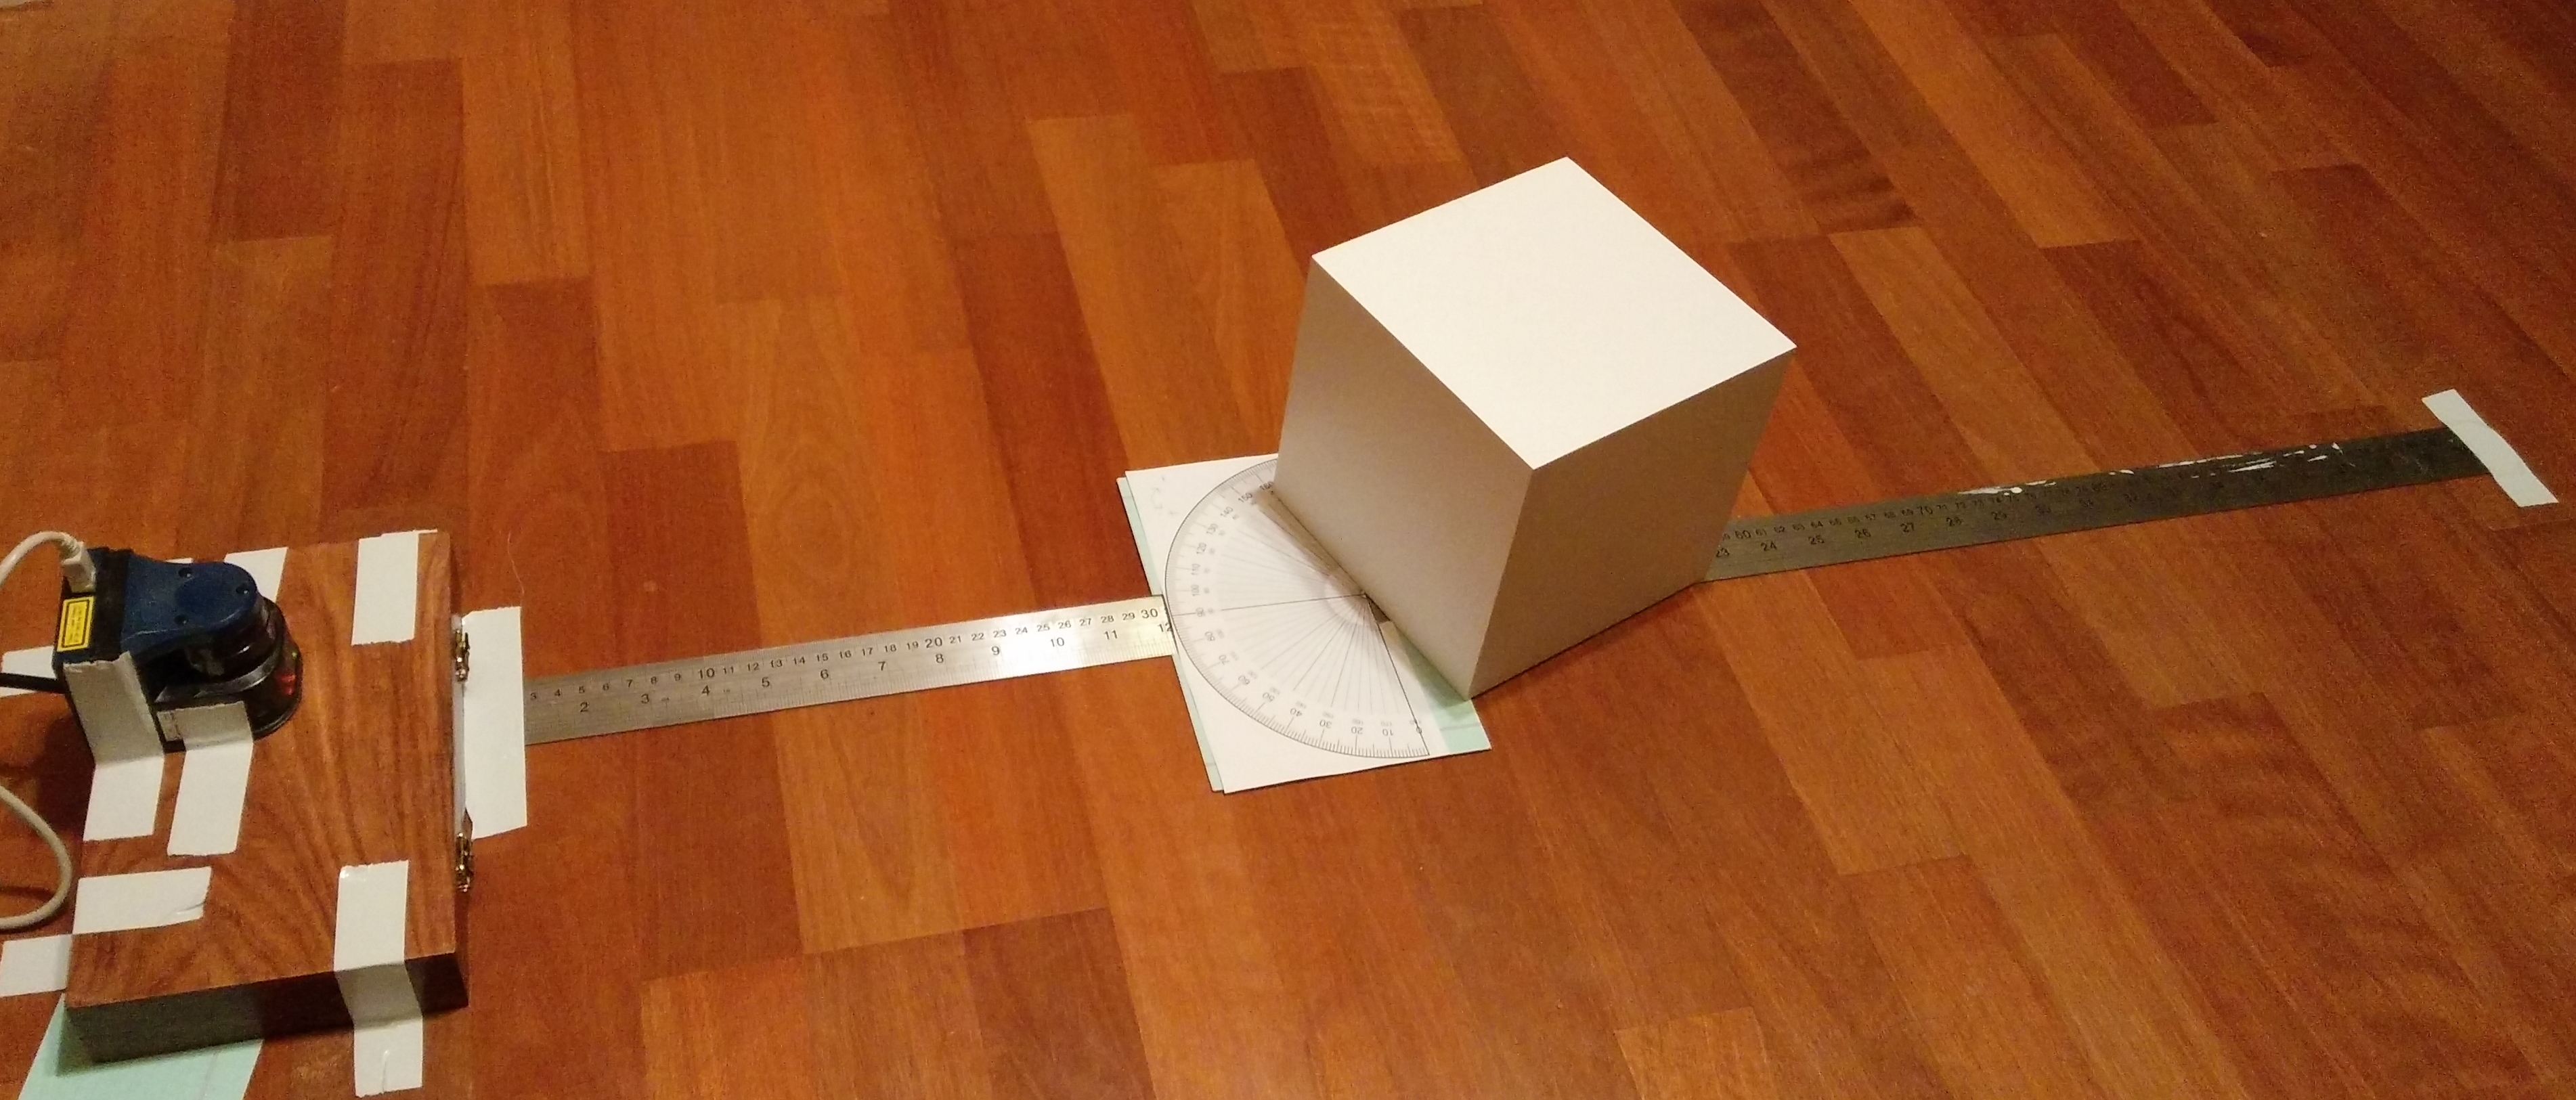
\includegraphics[width=1\textwidth,trim = 0mm 0mm 0mm 0mm,clip=true]{./Figures/noise_setup}\vspace*{0ex}
	  	\caption{setup to measure noise at a different ranges and angle (lights turned off during measurement to eliminate error from variation in lighting conditions)} \label{fig:noise_setup}
	\end{figure}
		 
	\subsection{Results}
		The range error $r_{error} = r_{ground truth} - r_{measured}$ was computed. The distributions of this error for varying ranges and angles is shown in Figure \ref{fig:mean_hist}. The range error is approximately normally distributed.
		\begin{figure}
		\centering
		  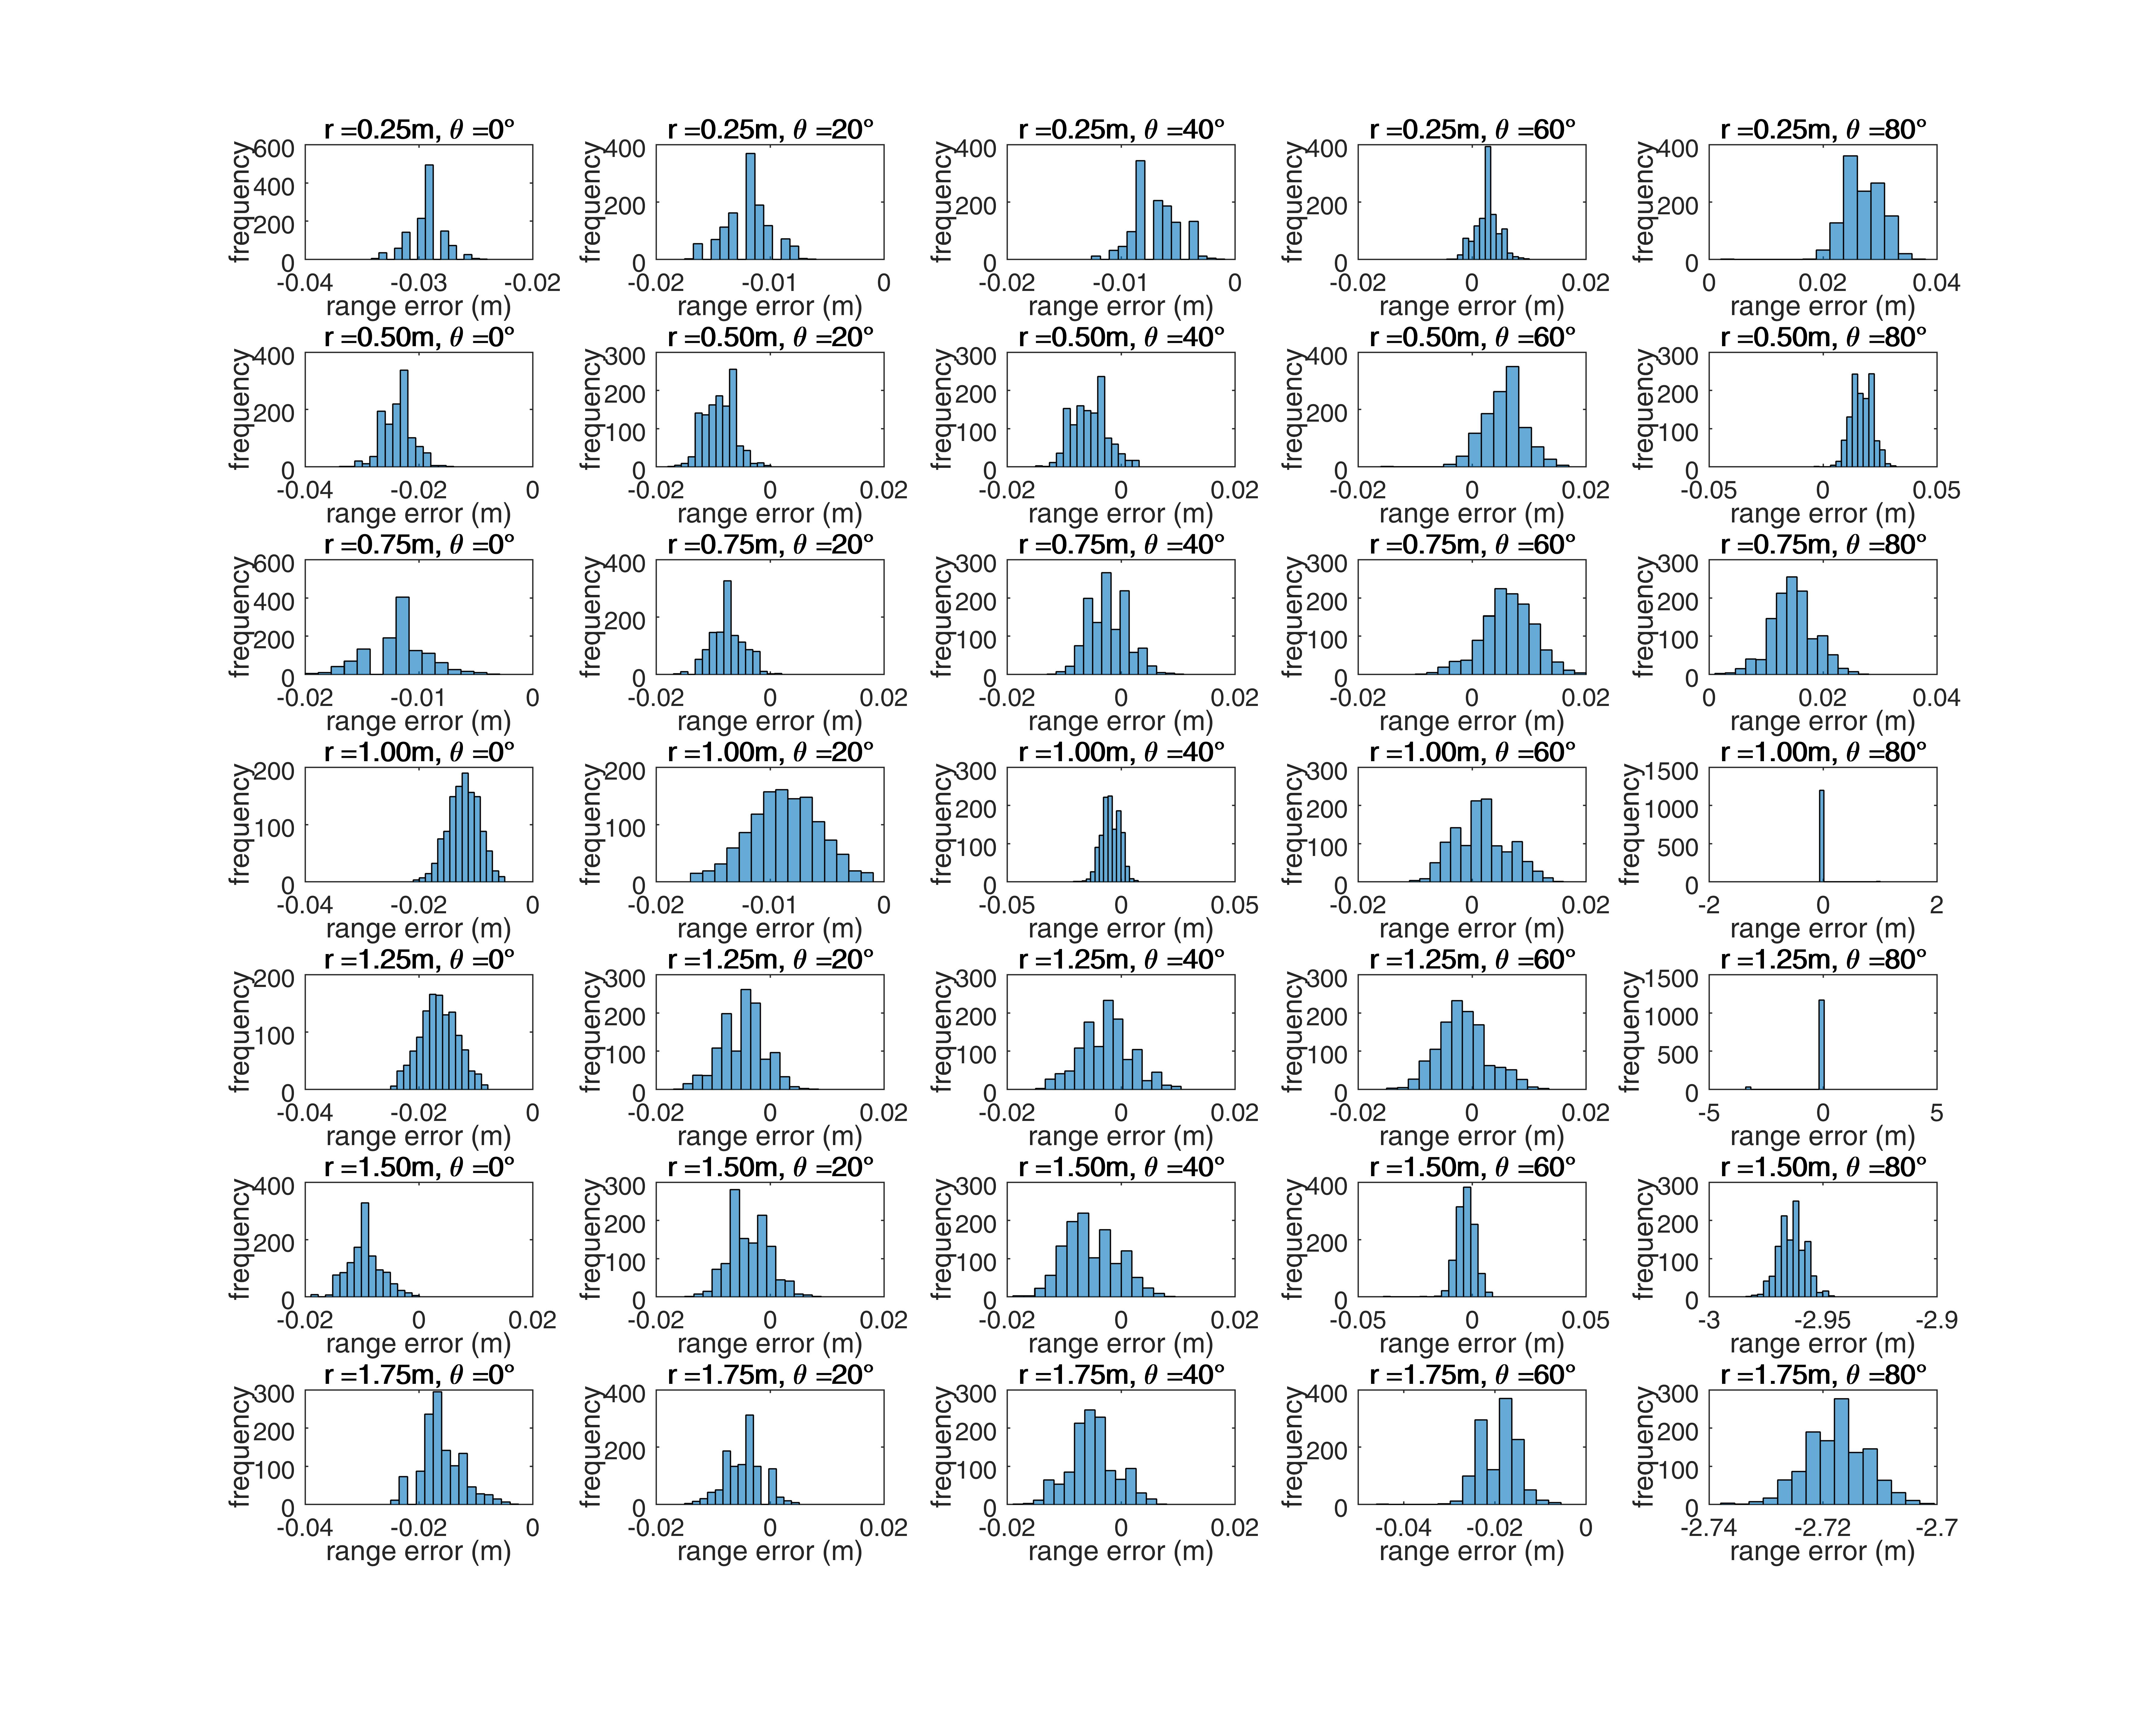
\includegraphics[width=1\textwidth,trim = 0mm 0mm 0mm 0mm,clip]{./Figures/range_error_histograms.jpg}
		  \caption{Sensor noise function $f_{UBG}(r,\theta)$ approximately normally distributed}
		  \label{fig:mean_hist}
		\end{figure}
		
		The mean range error as function of $r$ and $\theta$ is shown in Figure \ref{fig:mean_range_error}. The standard deviation of the range errors as function of $r$ and $\theta$ is shown in Figure \ref{fig:stddev_range_error}.
		\begin{figure}
	  		\centering
	  		\subfigure[\label{fig:mean_range_error_outliers}]{
	  		\begin{minipage}[b]{0.45\columnwidth}
    			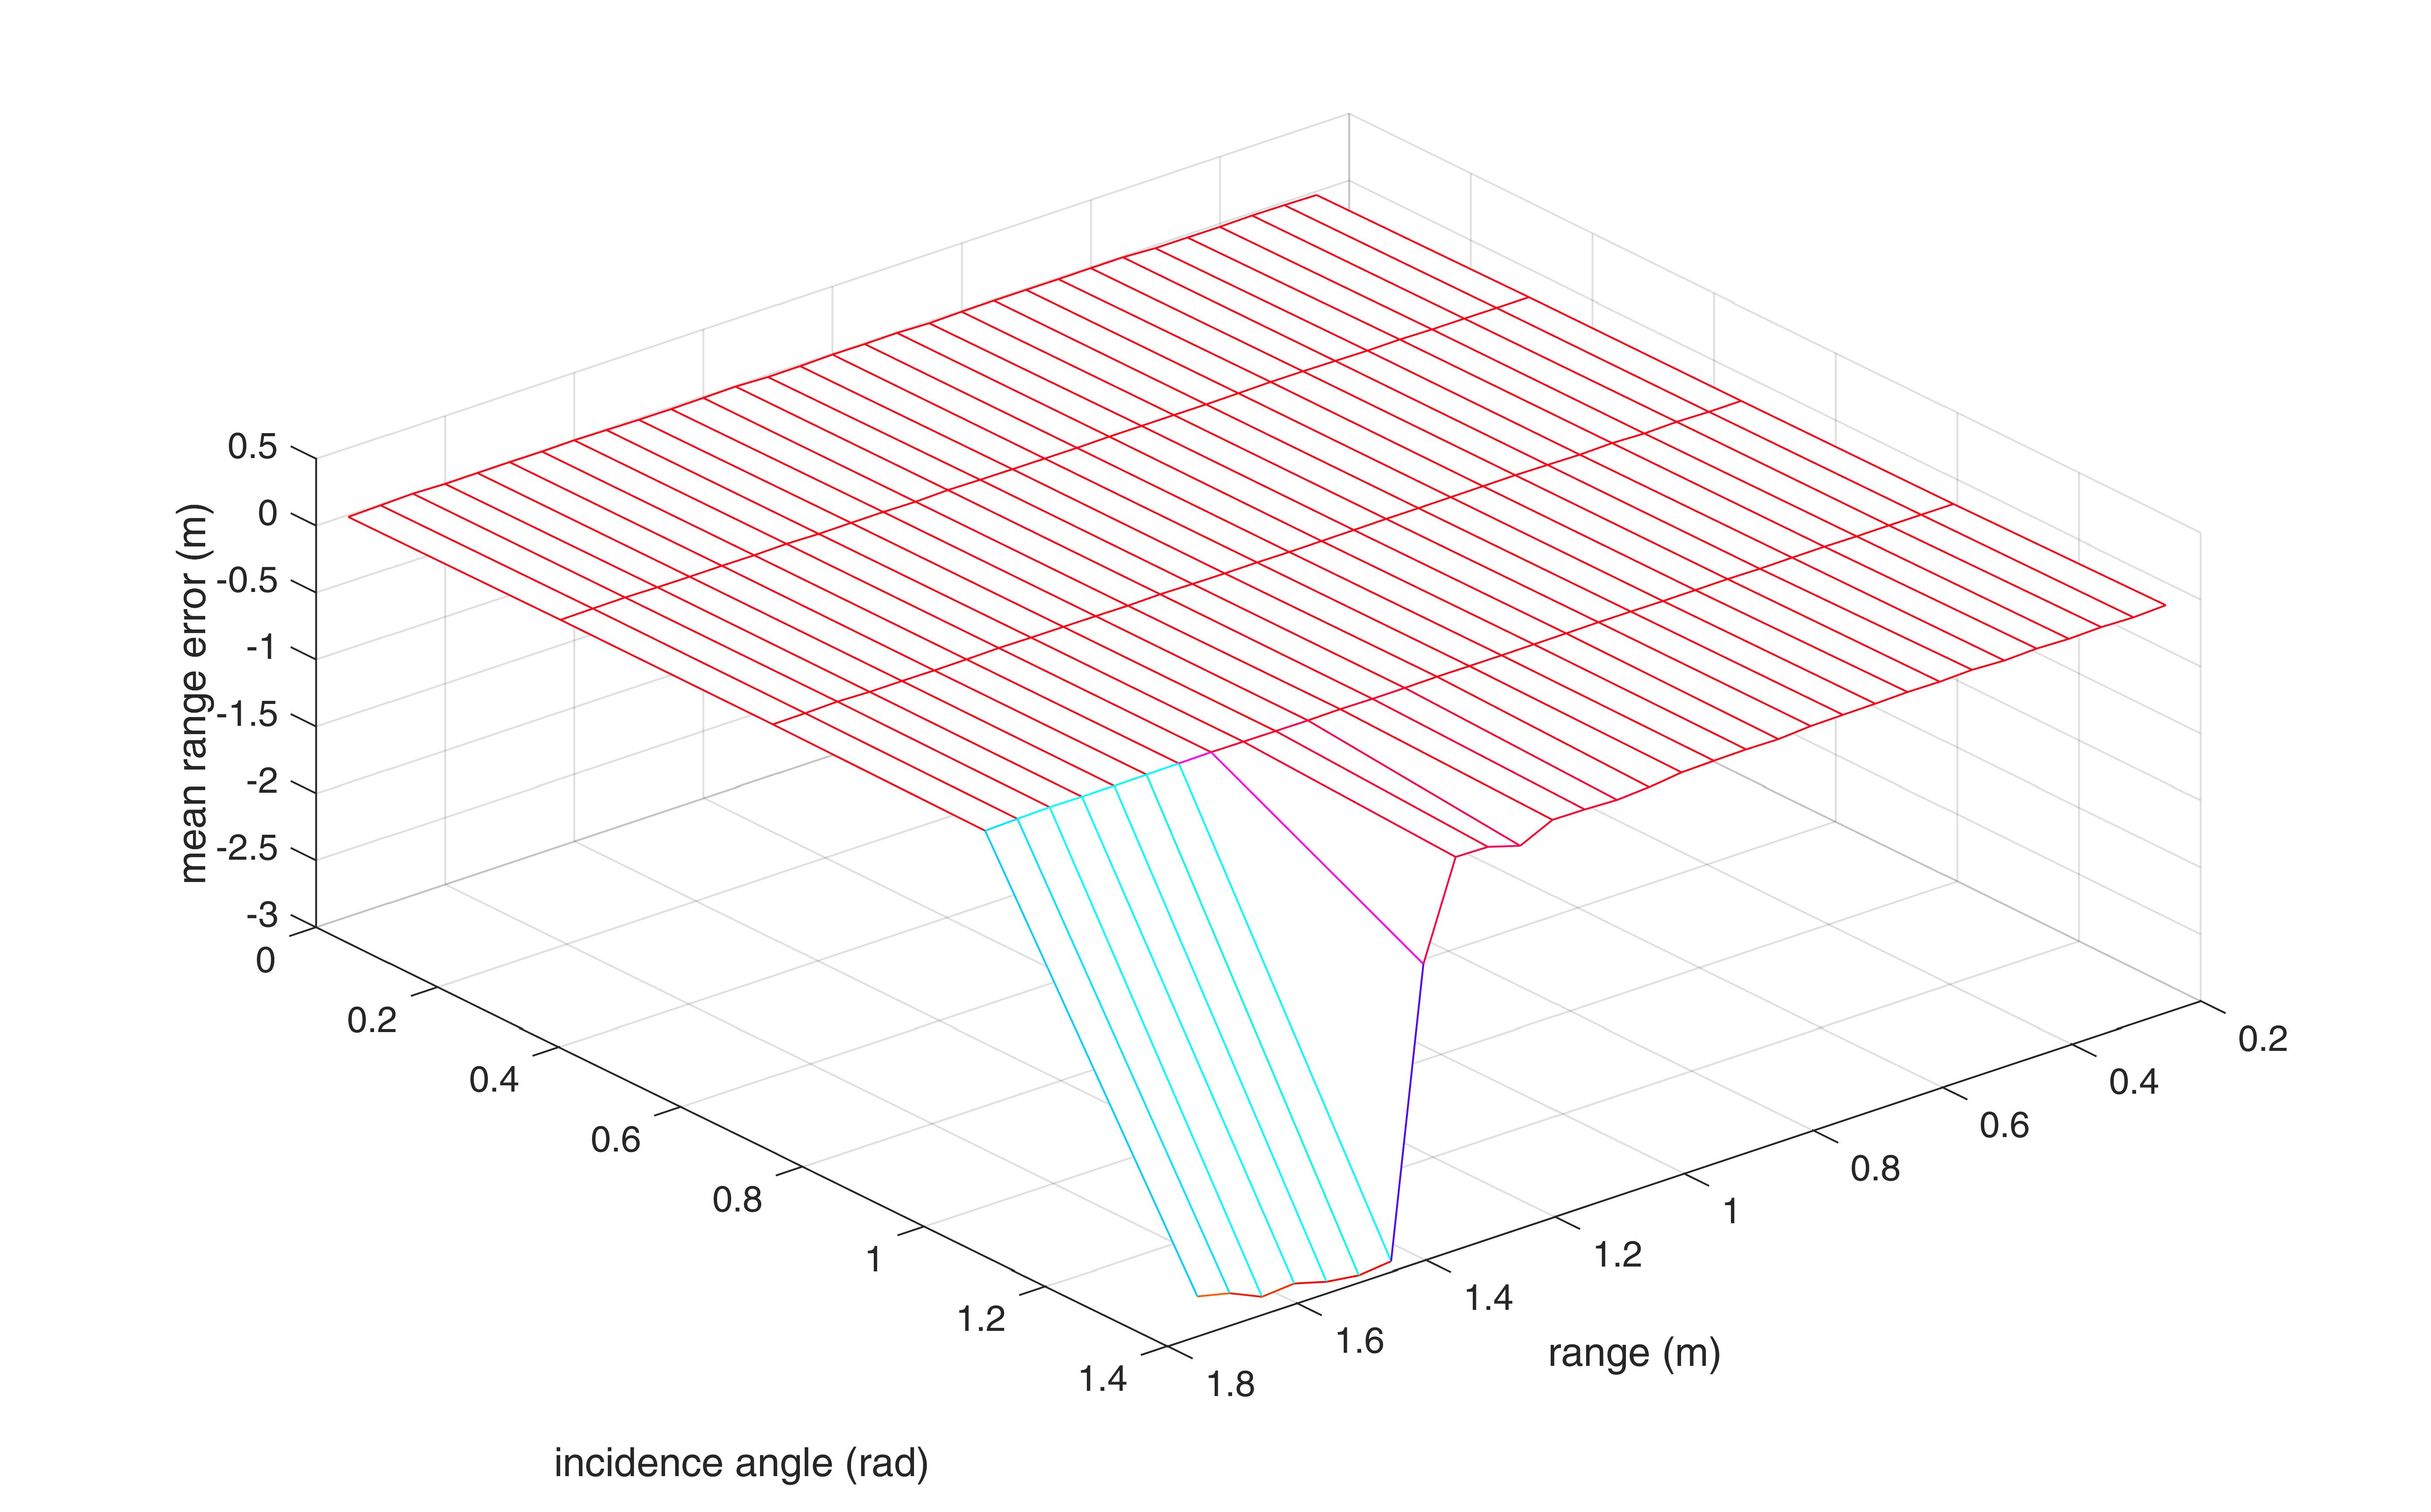
\includegraphics[width=1\textwidth,trim = 0mm 0mm 0mm 0mm,clip]{./Figures/noise_mean_range_error}\vspace*{0ex}
	  		\end{minipage}}
	  		\subfigure[\label{fig:mean_range_error_no_outliers}]{
	  		\begin{minipage}[b]{0.45\columnwidth}
    			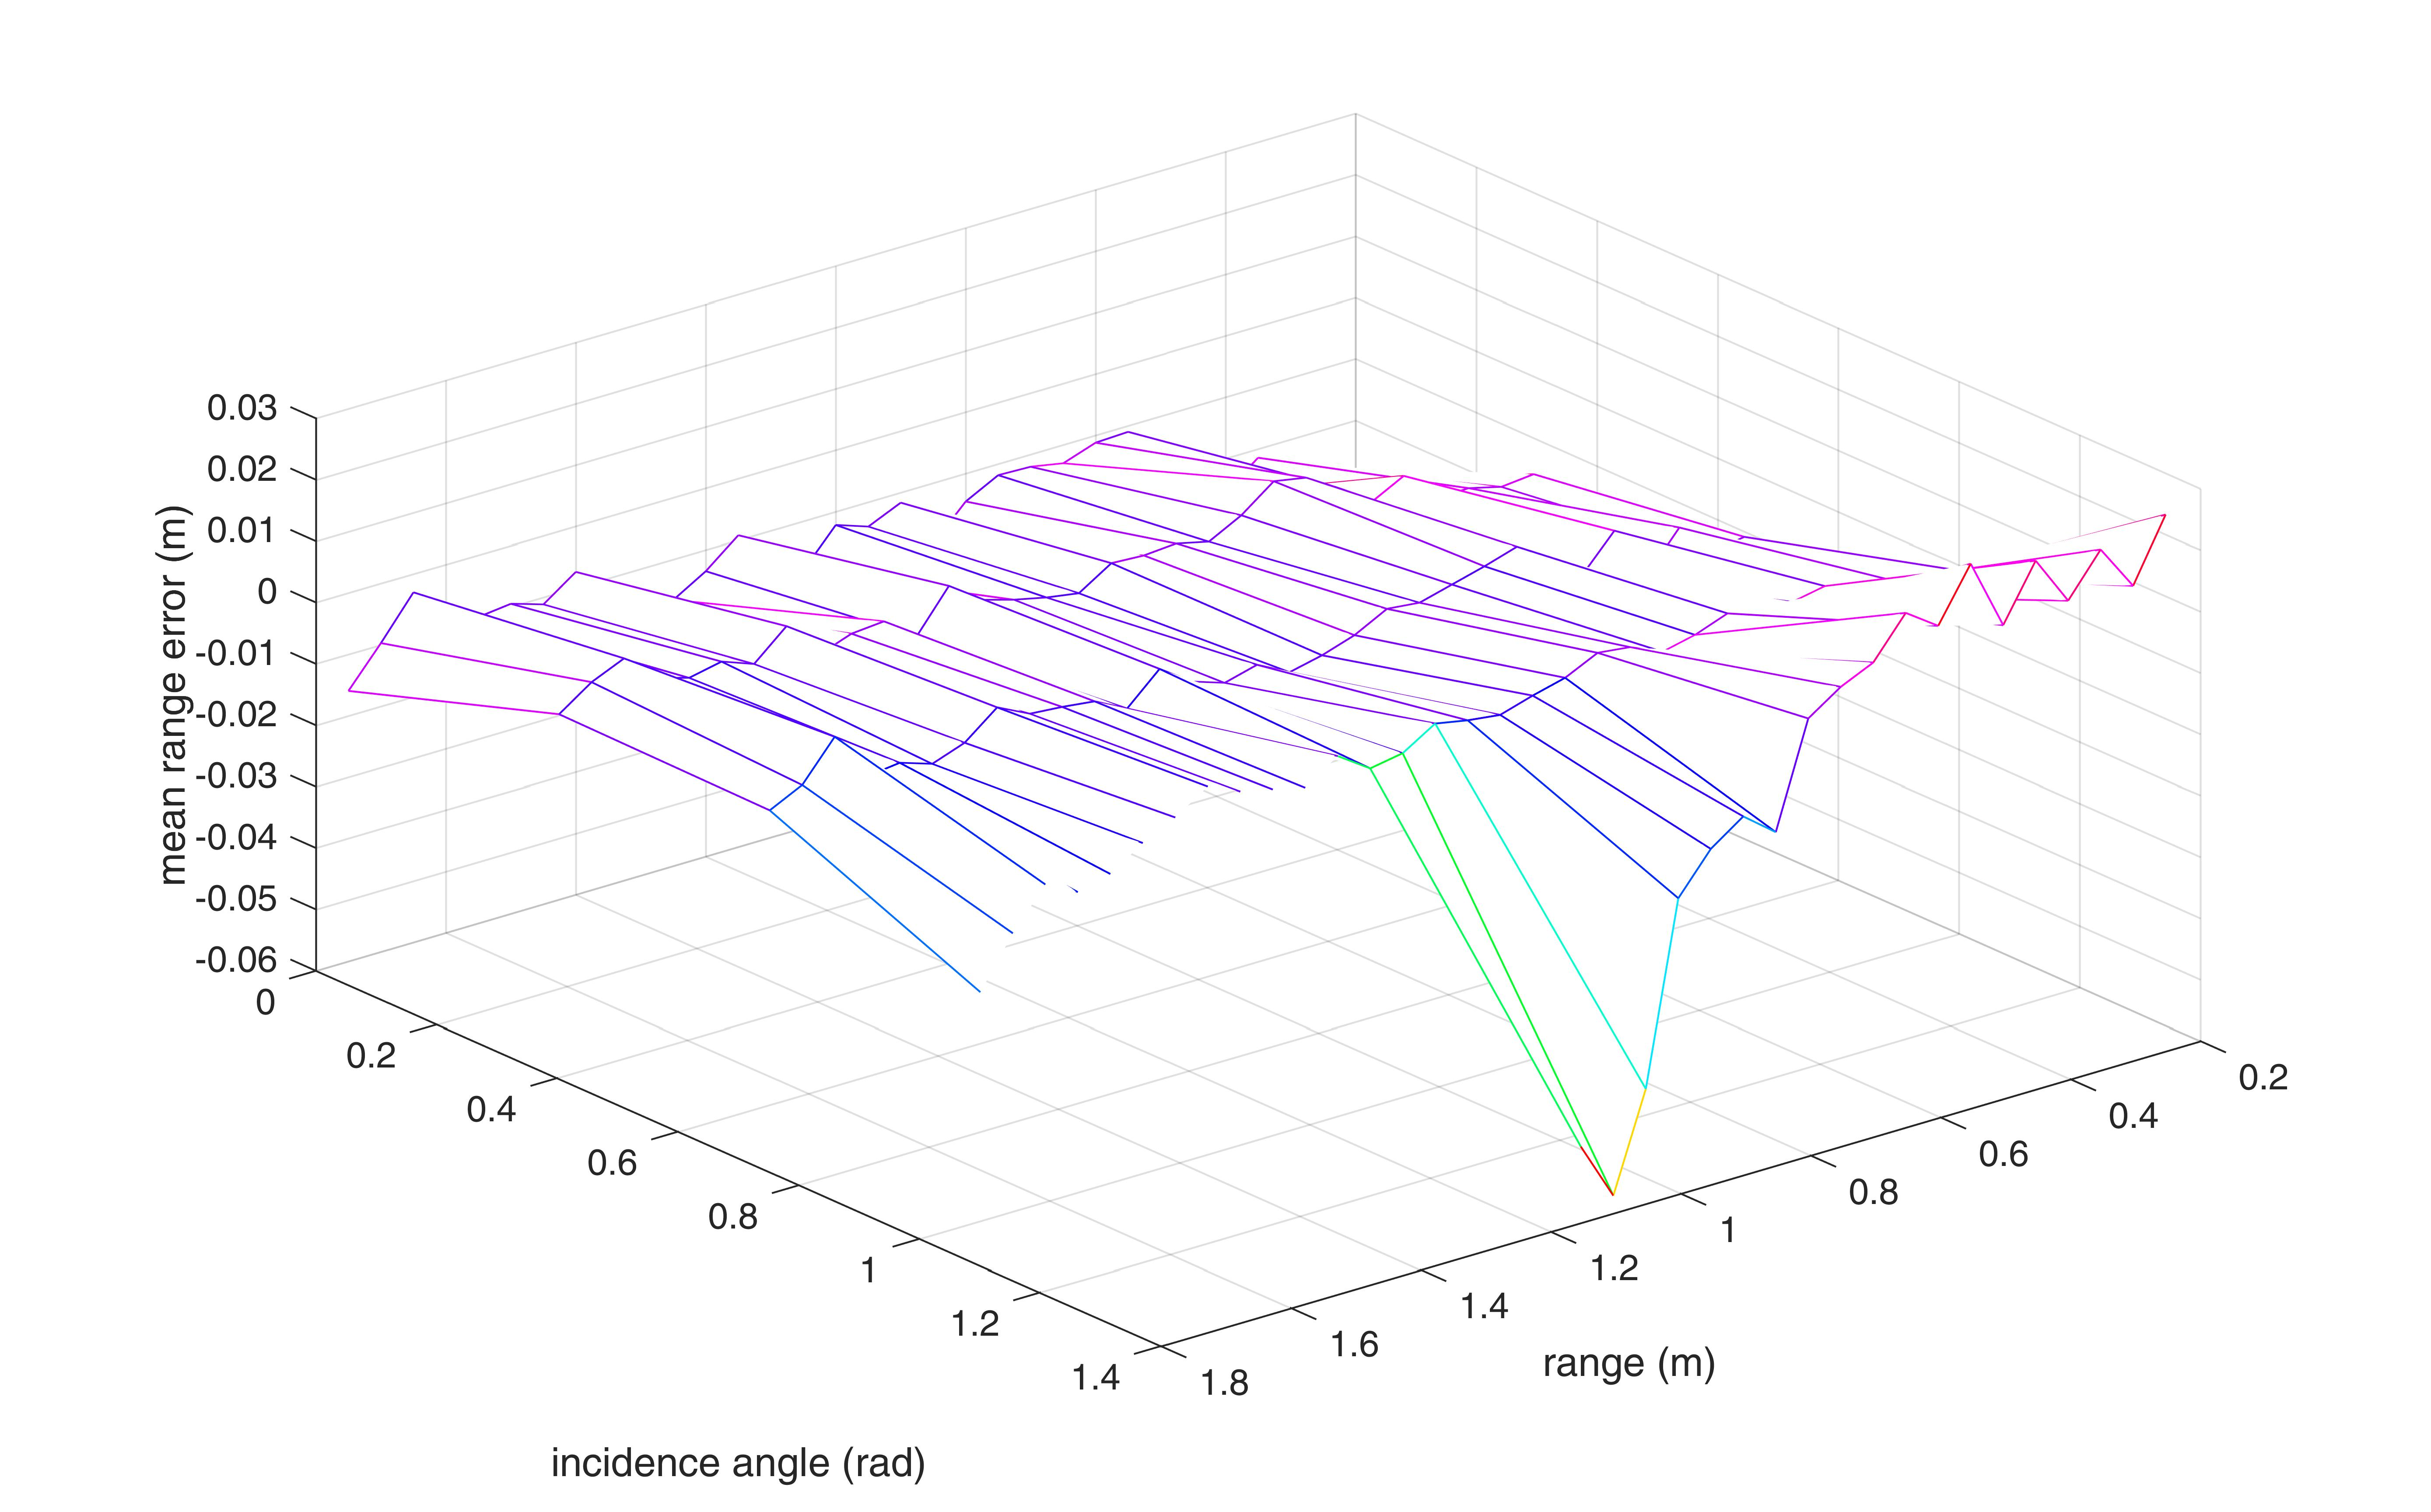
\includegraphics[width=1\textwidth,trim = 0mm 0mm 0mm 0mm,clip]{./Figures/noise_mean_range_error_removed_outliers}\vspace*{0ex}
		 \end{minipage}}
	  		\caption{mean range error ($r_{error} = r_{ground truth} - r_{measured}$) vs $(r,\theta)$ showing (a) large error at high angles and range, (b) overall shape}
	  		\label{fig:mean_range_error}
		\end{figure}
		
		\begin{figure}
	  		\centering
	  		\subfigure[\label{fig:stddev_range_error_outliers}]{
	  		\begin{minipage}[b]{0.45\columnwidth}
    			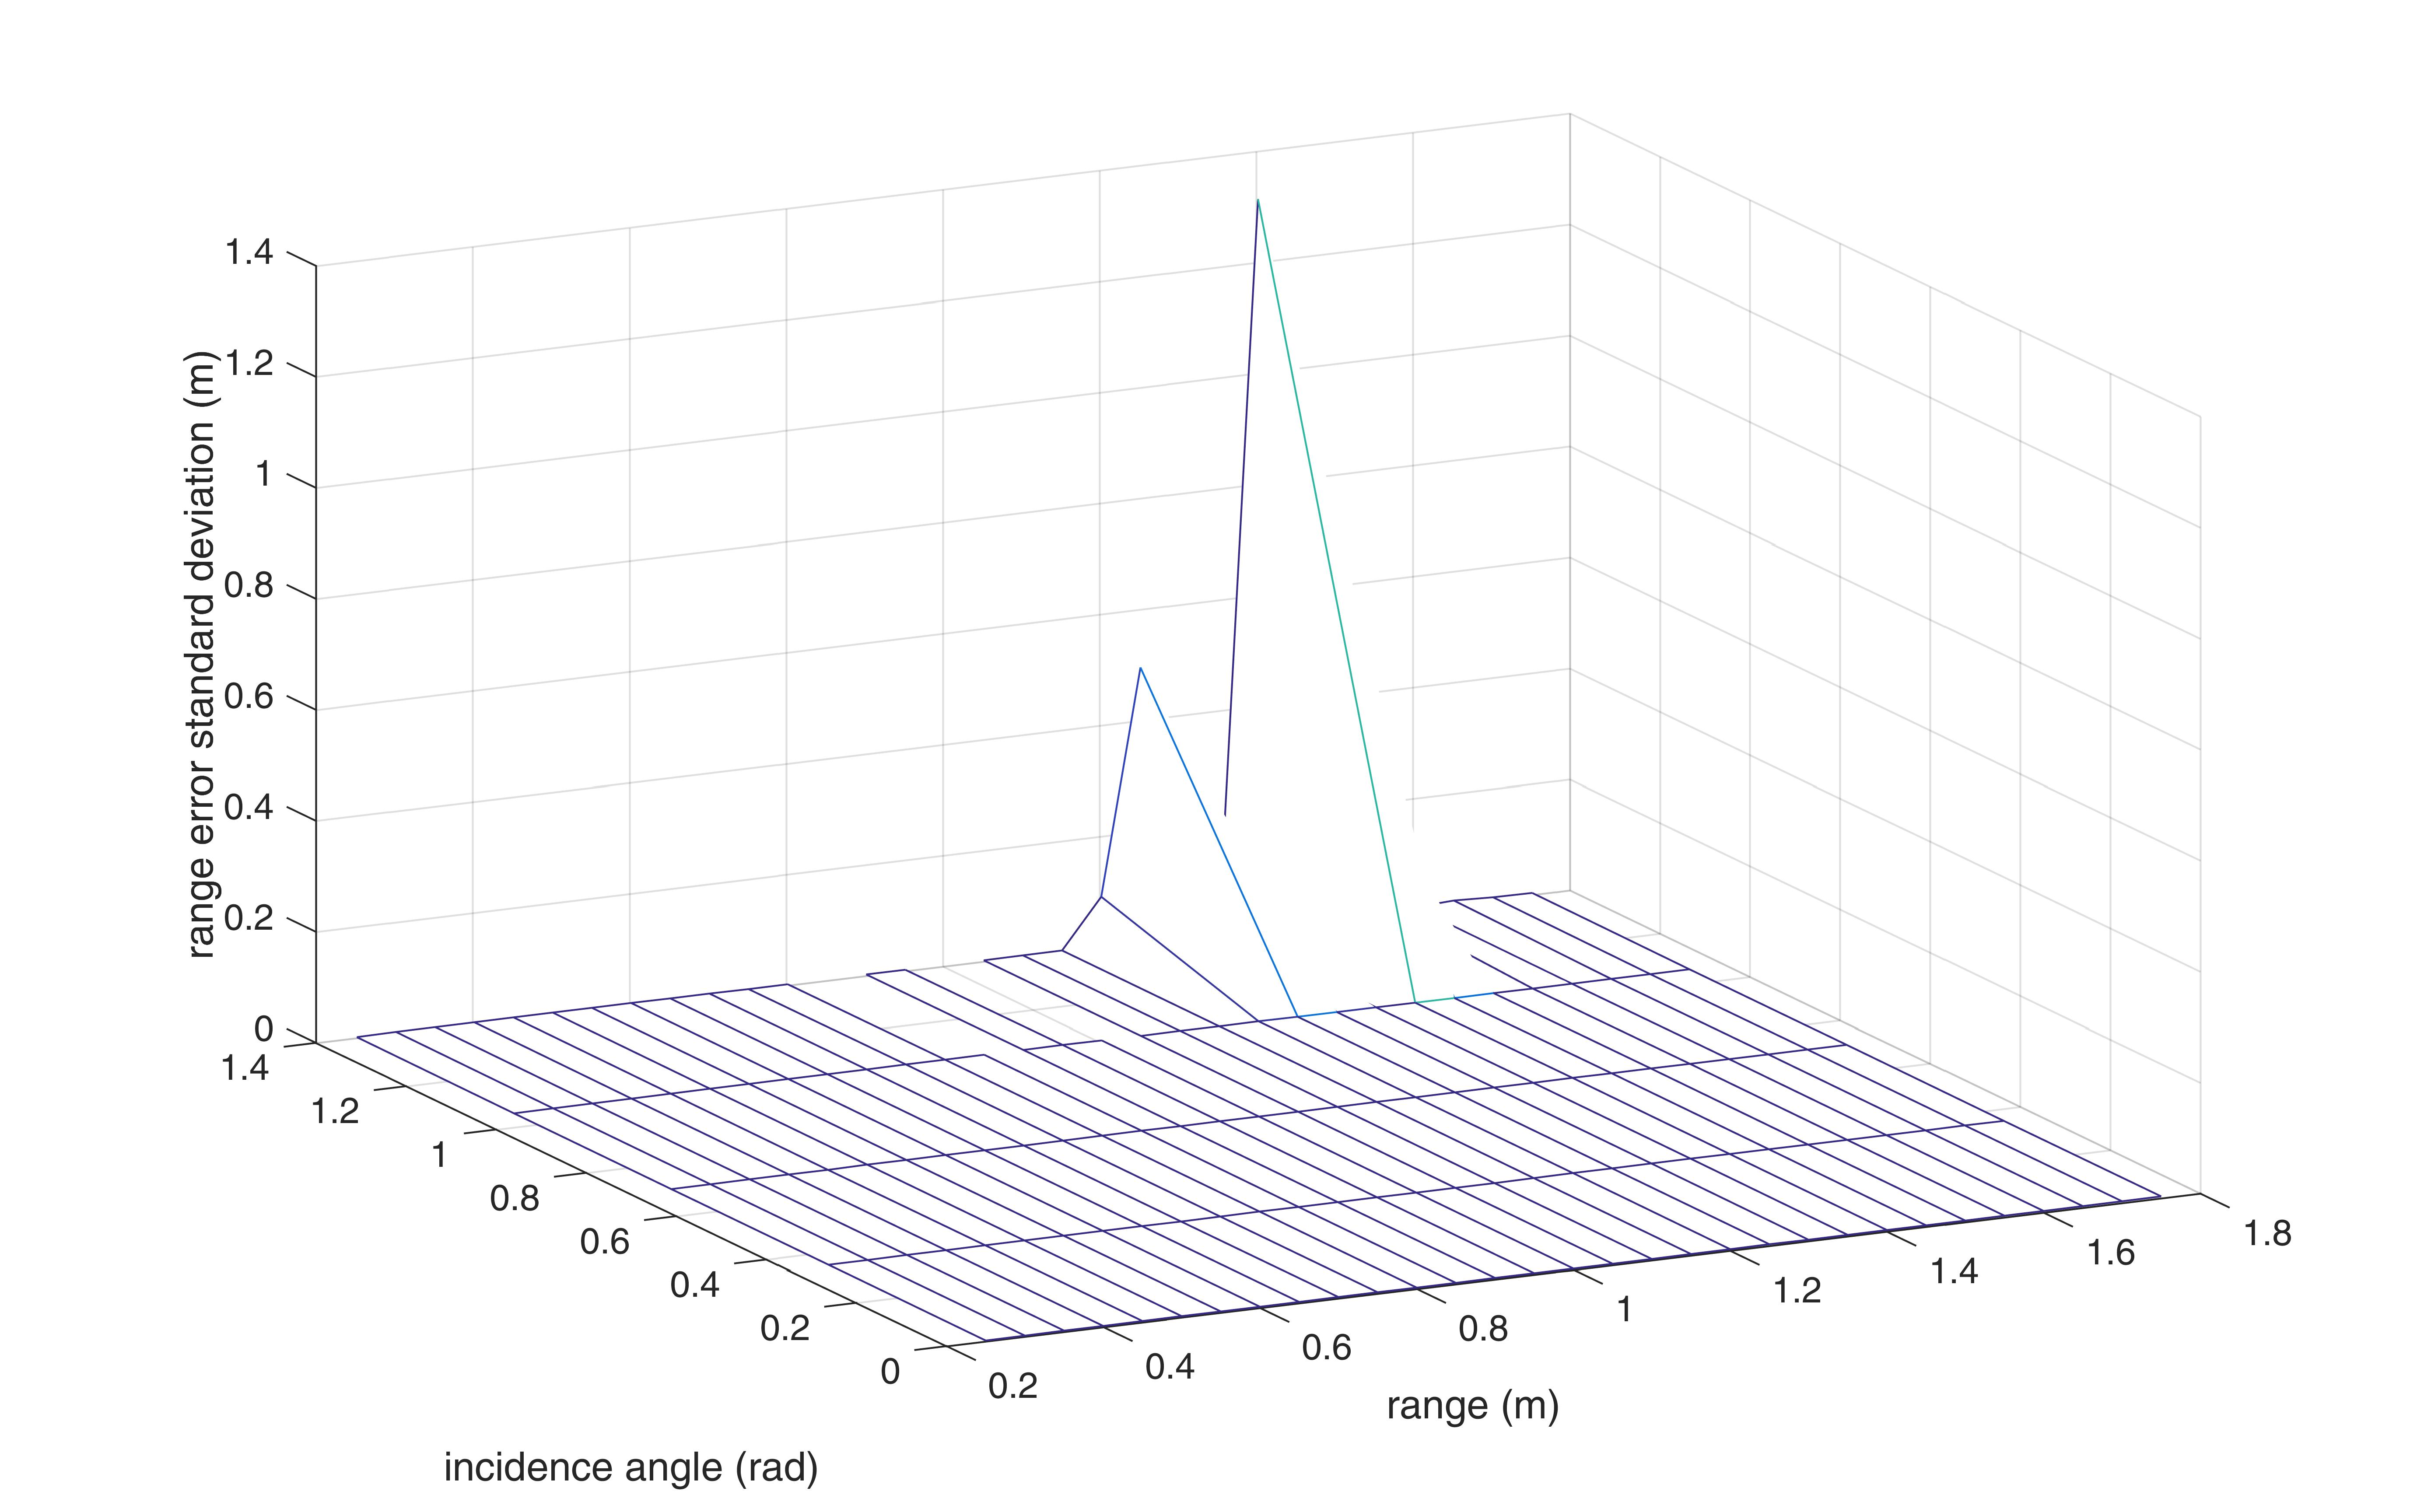
\includegraphics[width=1\textwidth,trim = 0mm 0mm 0mm 0mm,clip]{./Figures/noise_stddev_range_error}\vspace*{0ex}
	  		\end{minipage}}
	  		\subfigure[\label{fig:stddev_range_error_no_outliers}]{
	  		\begin{minipage}[b]{0.45\columnwidth}
    			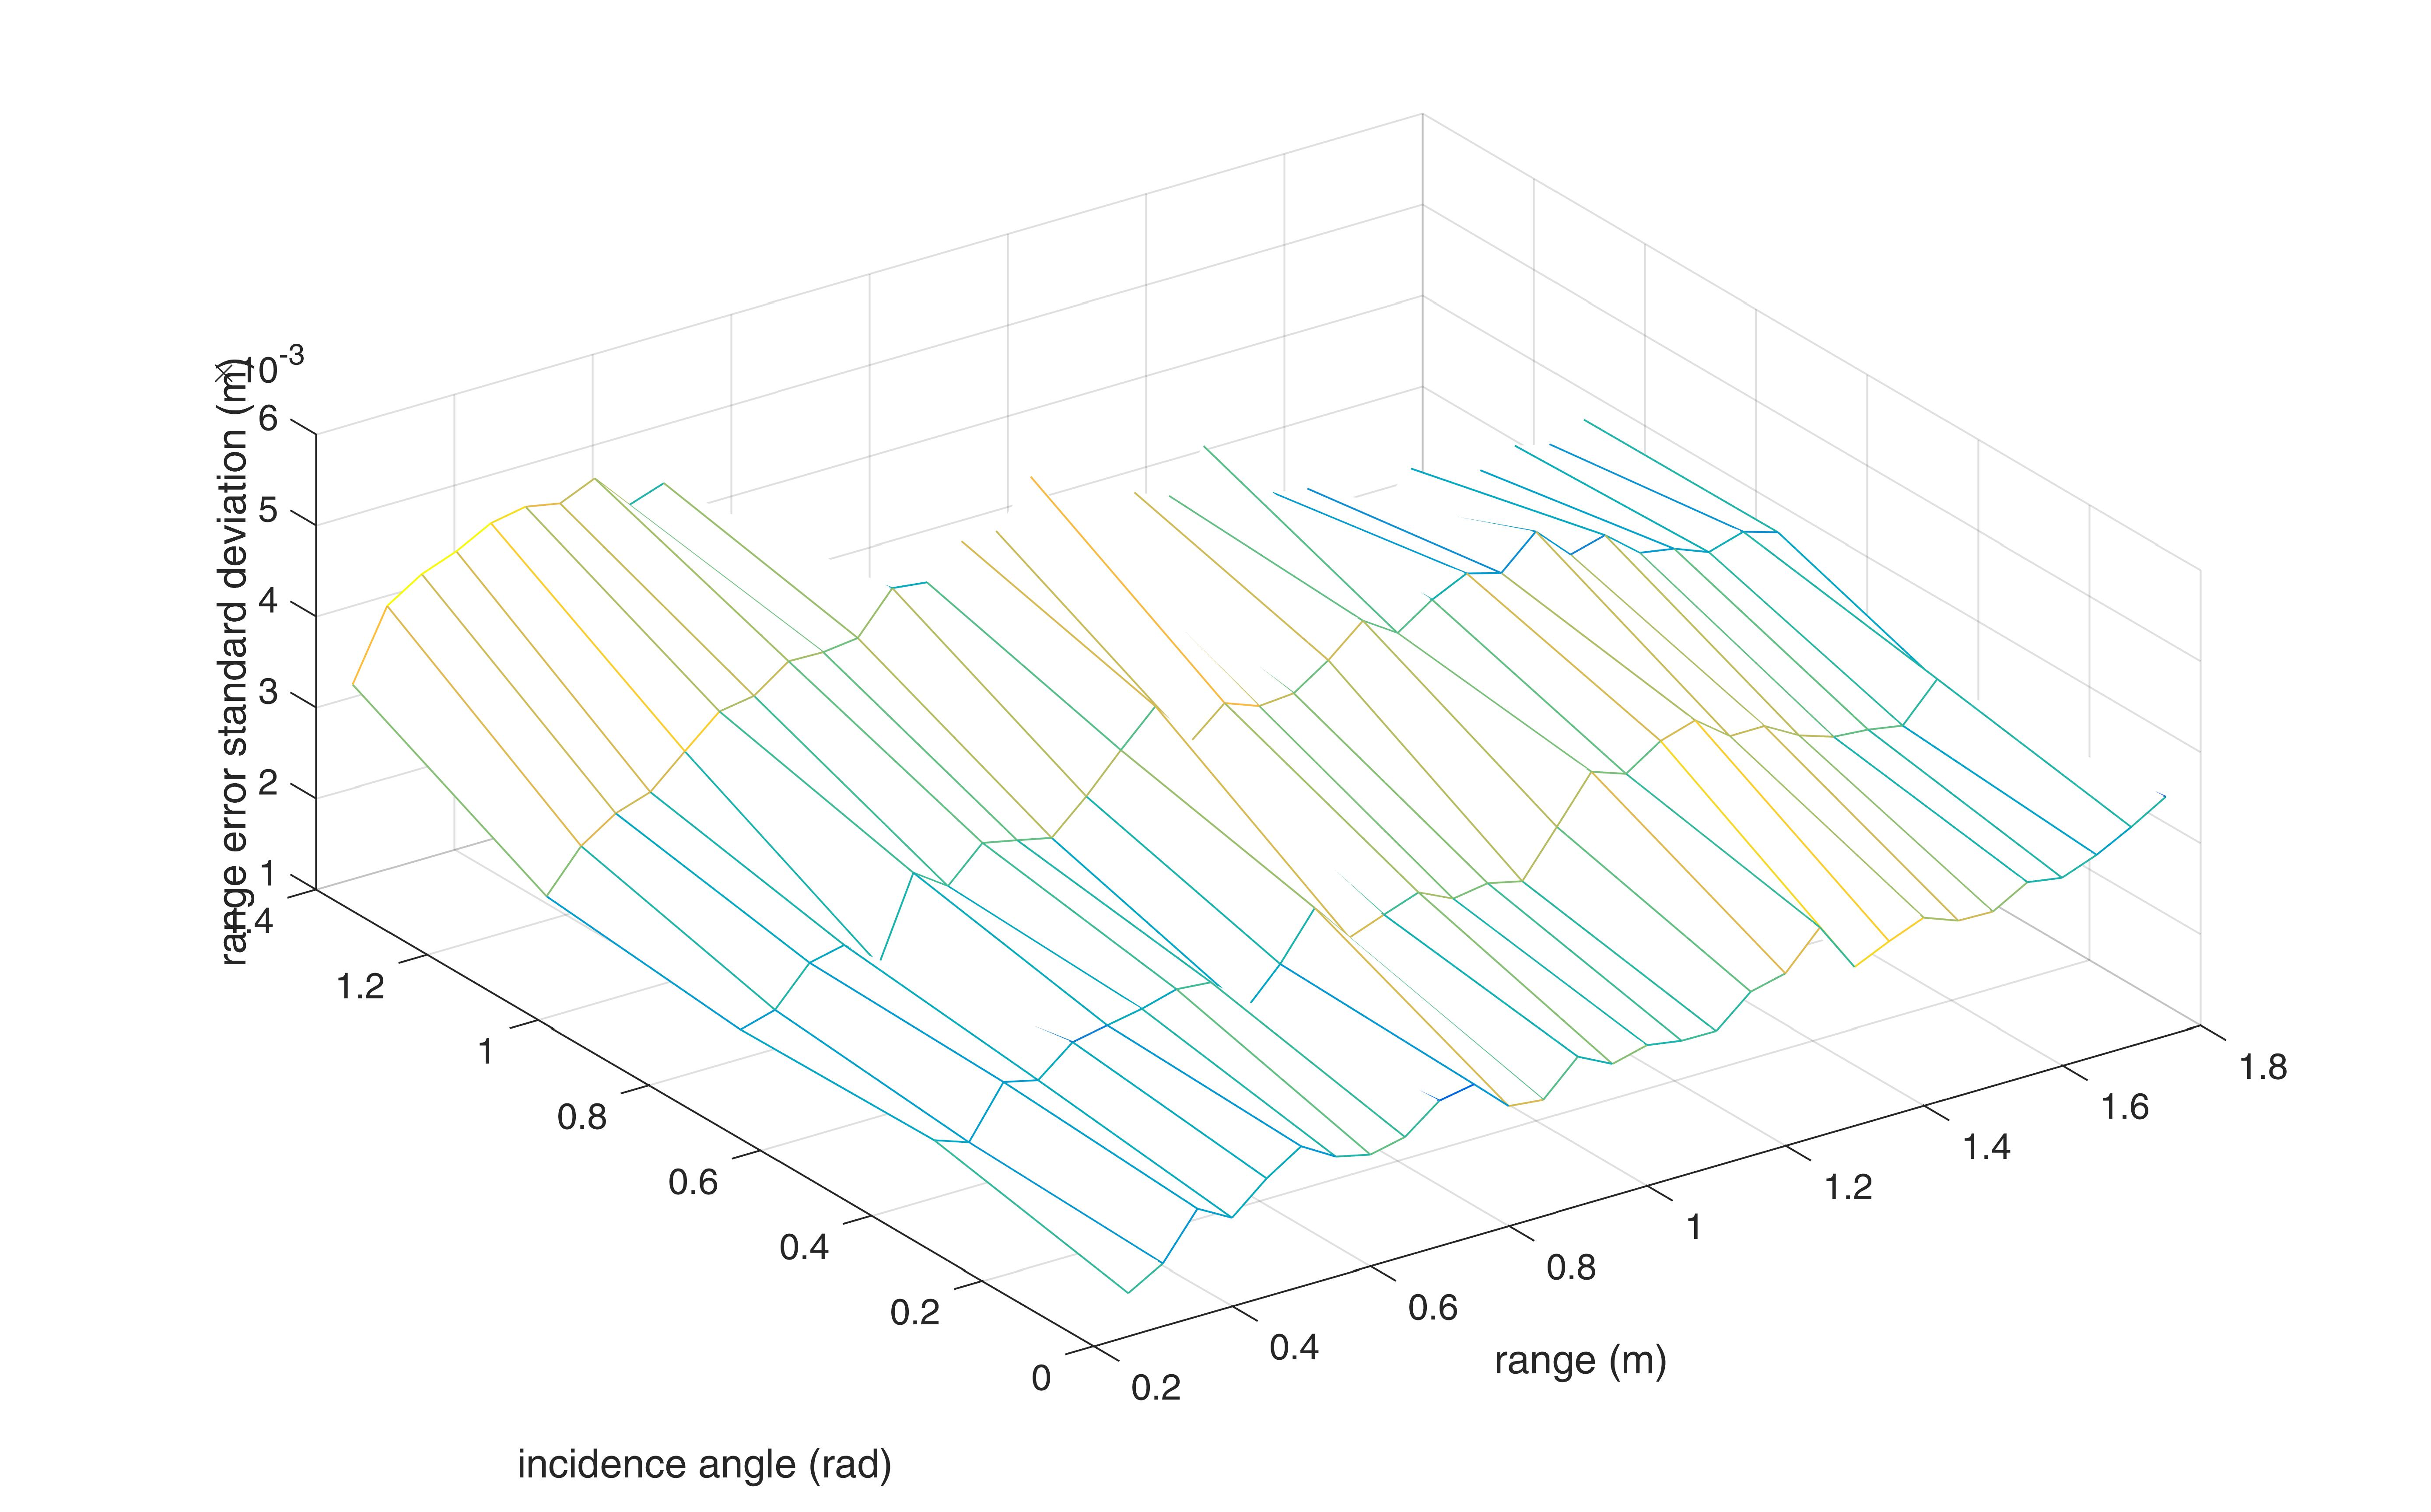
\includegraphics[width=1\textwidth,trim = 0mm 0mm 0mm 0mm,clip]{./Figures/noise_stddev_range_error_removed_outliers}\vspace*{0ex}
	 		 \end{minipage}}
	  		\caption{range error $\sigma$ vs $(r,\theta)$ showing (a) outliers/large std dev at high angles and range, (b) overall shape}
	  		\label{fig:stddev_range_error}
		\end{figure}
		
		Figures \ref{fig:mean_range_error_outliers} and \ref{fig:stddev_range_error_outliers} show that the mean error and error standard deviation increase significantly when $\theta > 75^\circ$ and $r > 0.8$m. This can be explained by considering what happens to the laser beam under these conditions. Though it has been idealised as a ray in the simulation, the laser has a nonzero beam width. Thus, as $\theta$ increases, one side of the beam will encounter the surface before the centre of the beam. A portion of the light will reach the sensor earlier, though the total amount of light will be reduced as the angle increases. This earlier reflected light will result in a shorter range measurement, but less reflected light will cause a longer range measurement. For angles greater than 75$^\circ$ and ranges greater than 0.8m, the reflected light is insufficient to allow a range measurement. The sensor returns the maximum possible range measurement of 4095mm. In modelling the noise, range measurements for $\theta > 75^\circ$ and $r > 0.8$m are discarded.
		
		These results are corroborated by \cite{park2010characterization} who reported difficulty in acquiring measurements for high angles and modelled the noise distribution as Gaussian.
		
		It was assumed that the noise distribution for an incidence angle $\theta$ would be identical to $-\theta$. However, the fact that the sensor's scan direction rotates in a single direction may mean this is not the case. Including the effect of incidence angles from $\pi/2$ to $\pi/2$ would provide a more accurate noise for future work.
		
		The 4th degree polynomial surfaces in equations \ref{eq:mean} and \ref{eq:std} were fitted to the adjusted set of data points using Matlab's curve fitting tool. The surfaces and the goodness of fit are shown in Figure \ref{fig:surface_range_error}. 
		\begin{figure}
	  		\centering
	  		\subfigure[\label{fig:surface_mean_range}]{
	  		\begin{minipage}[b]{0.45\columnwidth}
    			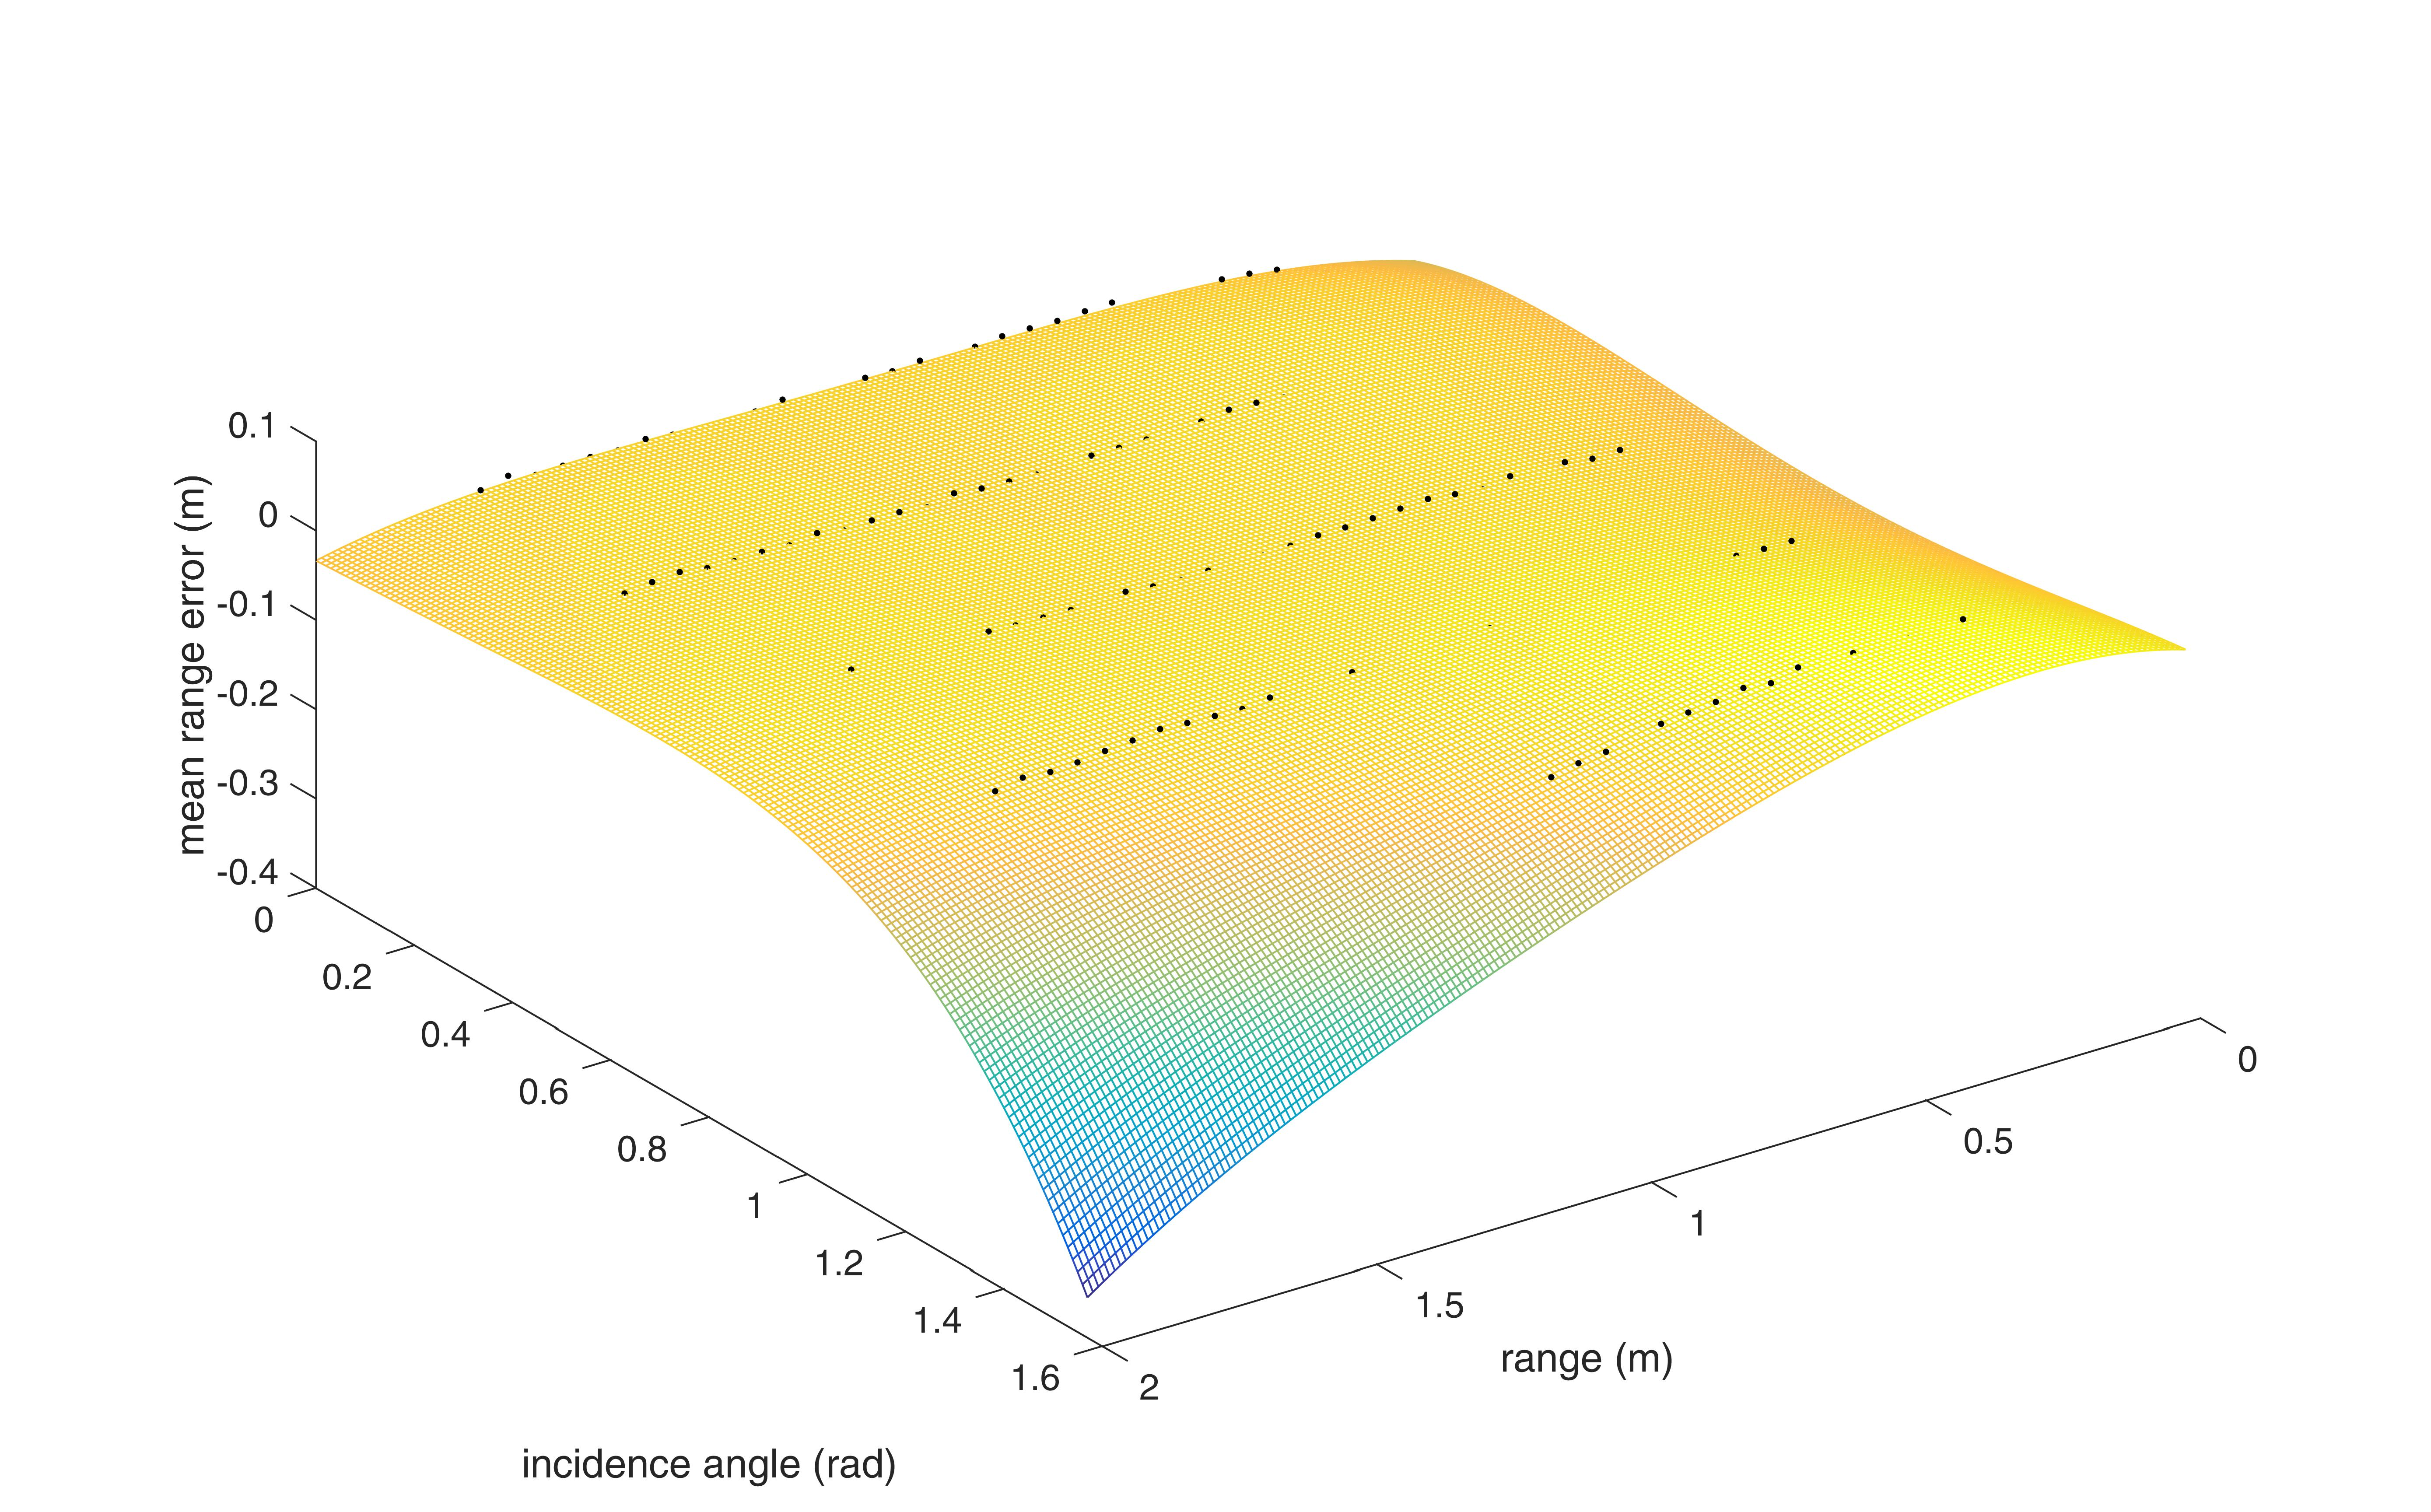
\includegraphics[width=1\textwidth,trim = 0mm 0mm 0mm 0mm,clip]{./Figures/surface_mean_range_error}\vspace*{0ex}
	  		\end{minipage}}
	  		\subfigure[\label{fig:surface_stddev_range}]{
	  		\begin{minipage}[b]{0.45\columnwidth}
    			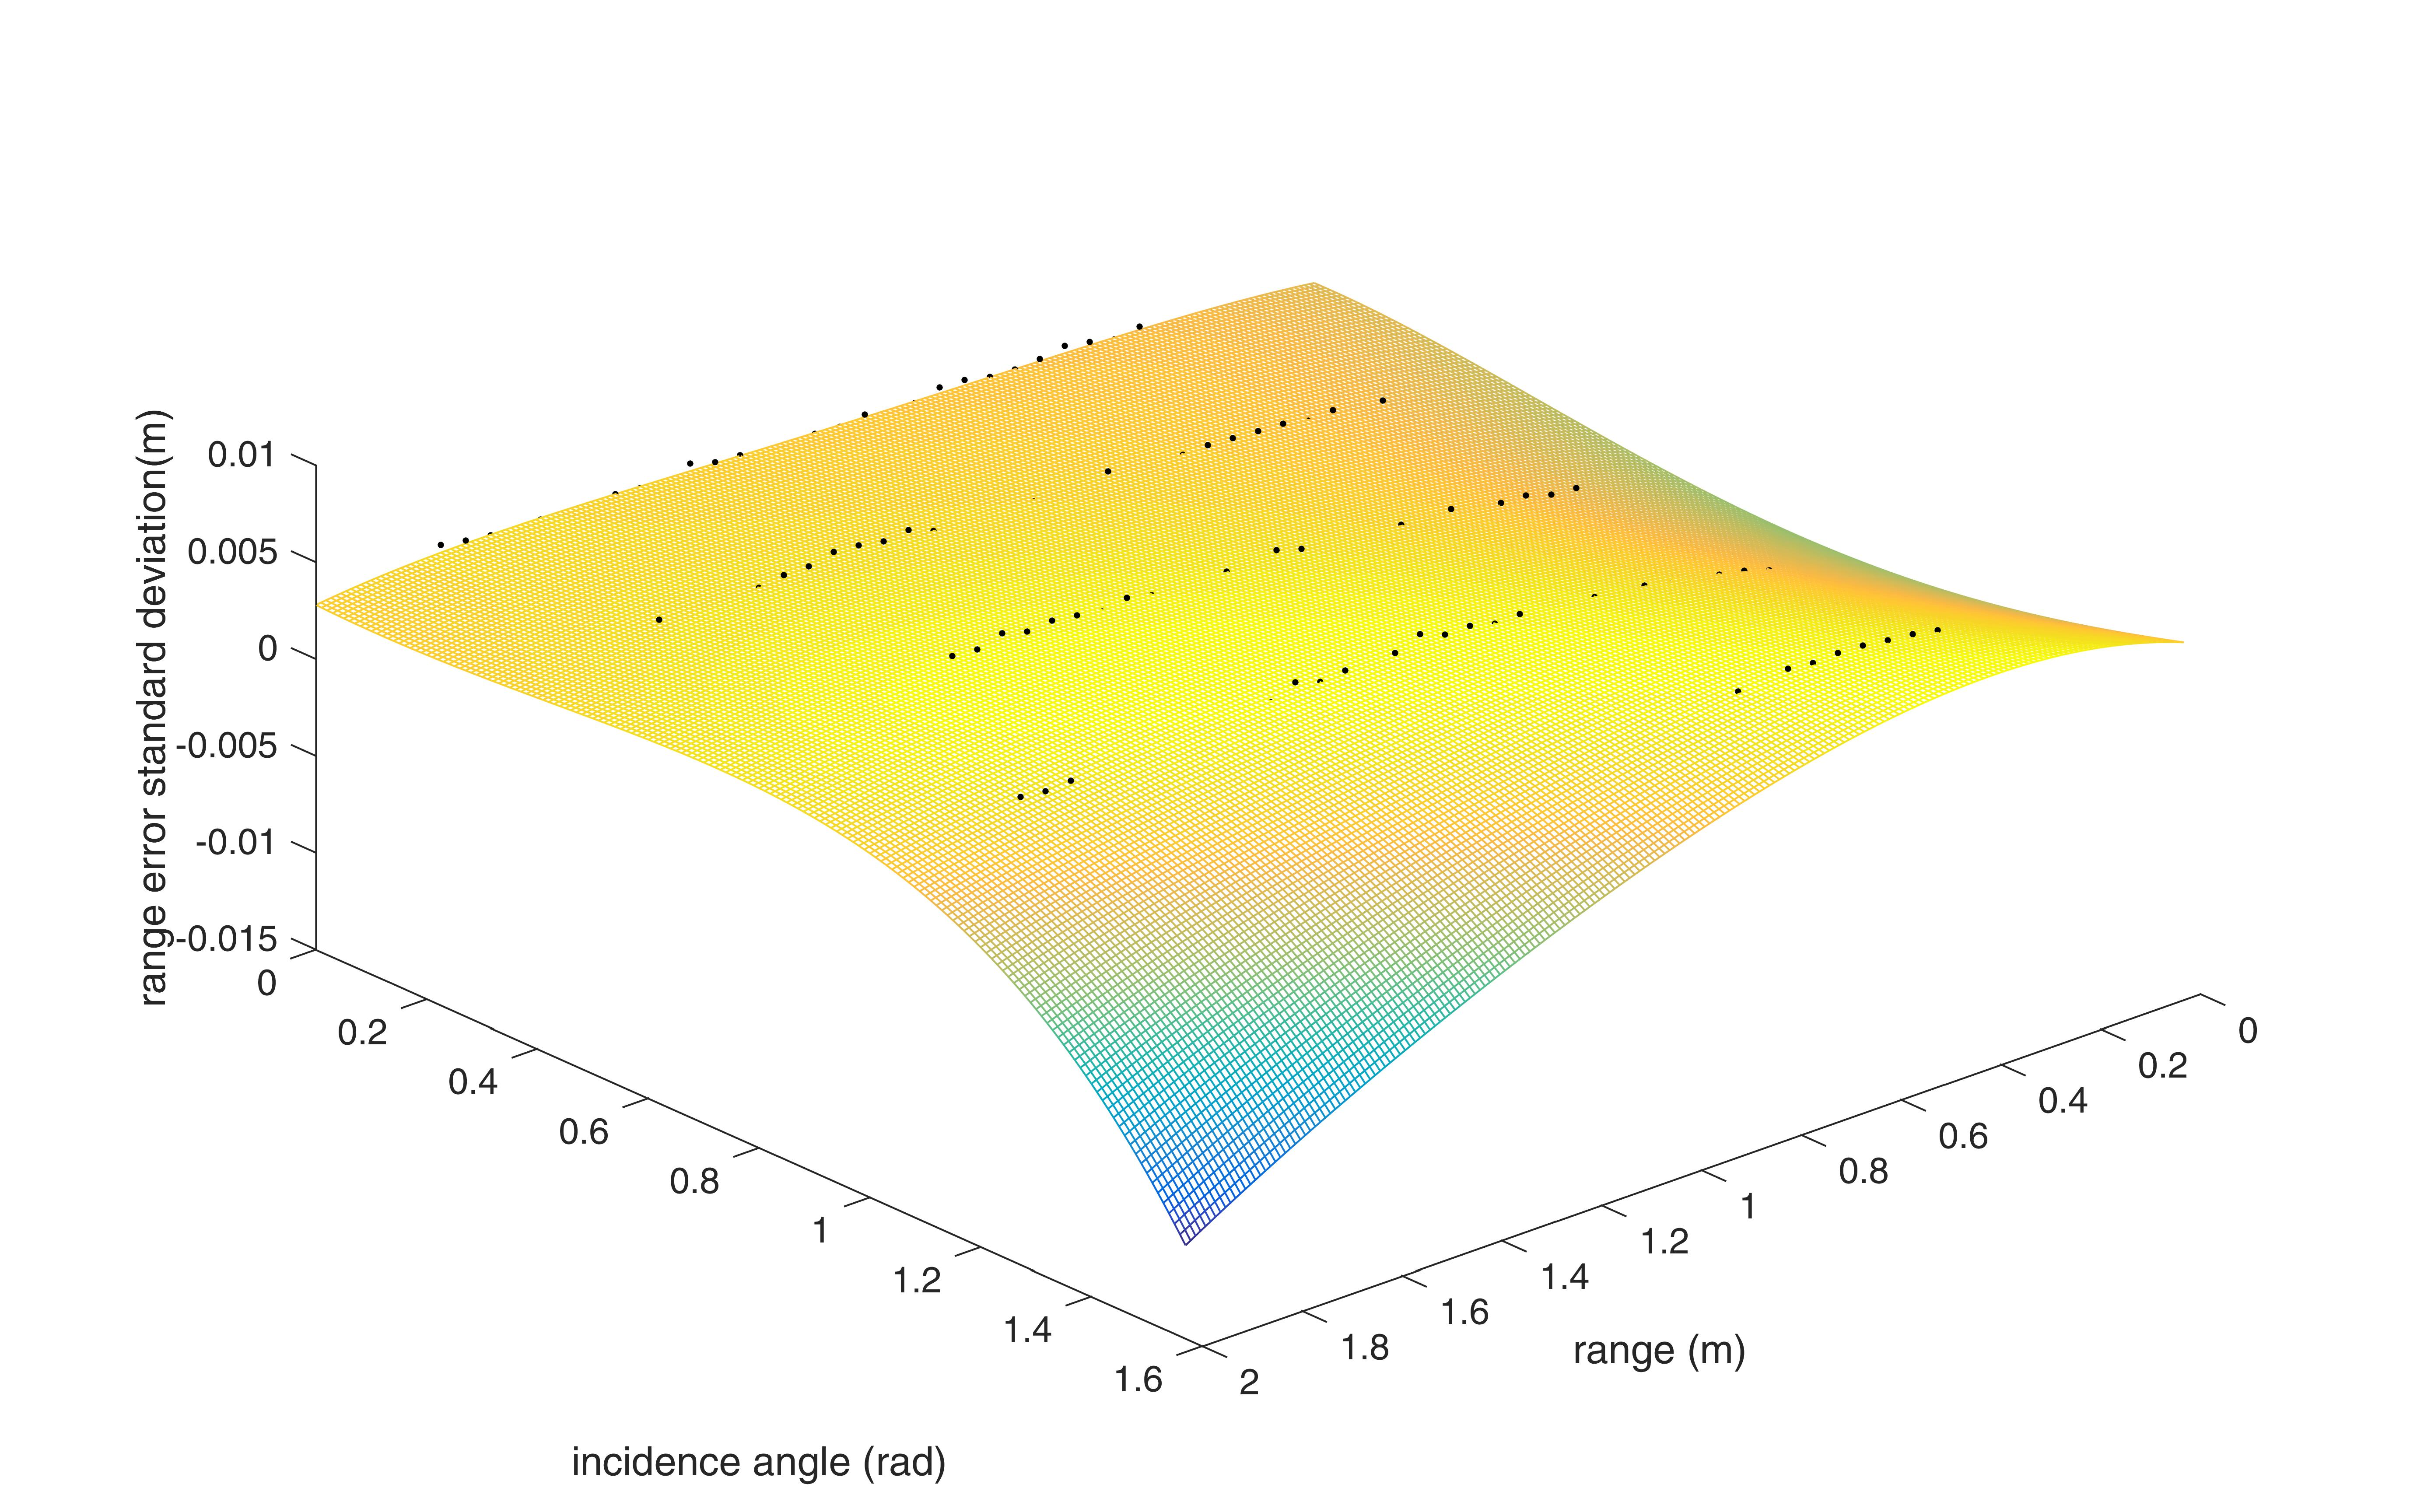
\includegraphics[width=1\textwidth,trim = 0mm 0mm 0mm 0mm,clip]{./Figures/surface_stddev_range_error}\vspace*{0ex}
		 \end{minipage}}
	  		\caption{polynomials fitted to range error mean \& standard deviation data points to model noise. (a) SSE: 0.003234, R-square: 0.8447, Adjusted R-square: 0.8278, RMSE: 0.005027(b) SSE: 7.592e-06, R-square: 0.9196, Adjusted R-square: 0.9103, RMSE: 0.0002515}
	  		\label{fig:surface_range_error}
		\end{figure}
		
		\subsubsection{Gaussian noise model}
		\begin{equation}
			\tilde{r}(r,\theta) = 
				\begin{cases}
					\hfill
					f_s(r,\theta,\phi(k)) = r + \mathcal{N}(\mu,\sigma)
						\hfill & \text{$\theta \leq 75^\circ$ or $r \leq 0.8$}\\
					NaN \hfill & \text{$\theta > 75^\circ$ and $r > 0.8$}
				\end{cases} 
		\end{equation}	
		where
		\begin{equation} \label{eq:mean}
			\begin{aligned}
				\mu = & a_{00} + a_{10}r + a_{01}\theta + a_{20}r^2 + a_{11}r\theta + a_{02}\theta^2\\
				      & + a_{30}r^3 + a_{21}r^2\theta + a_{12}r\theta^2 + a_{03}\theta^3 + a_{40}r^4 \\ 
				      & + a_{31}r^3\theta + a_{22}r^2\theta^2 + a_{13}r\theta^3 + a_{04}\theta^4
			\end{aligned}		
		\end{equation}
		\begin{equation} \label{eq:std}
			\begin{aligned}
				\sigma = & b_{00} + b_{10}r + b_{01}\theta + b_{20}r^2 + b_{11}r\theta + b_{02}\theta^2\\
			         	 & + b_{30}r^3 + b_{21}r^2\theta + b_{12}r\theta^2 + b_{03}\theta^3 + a_{40}r^4 \\ 
			         	 & + b_{31}r^3\theta + b_{22}r^2\theta^2 + b_{13}r\theta^3 + b_{04}\theta^4
			\end{aligned}
		\end{equation}
		
		and coefficients $a_{ij}$ and $b_{ij}$ are provided in tables \ref{tab:noise_a} and \ref{tab:noise_b} respectively.
				\begin{table}[h!]
  \centering
  \caption{$a_{ij}$ coefficients}
  \label{tab:noise_a}
  \begin{tabular}{c| c c c c c}
     	  & $j_0$ 	 & $j_1$   & $j_2$ 	 & $j_3$   & $j_4$ \\
    \hline
   	$i_0$ & -0.06529 & 0.2126  & -0.533	 & 0.4629  & -0.1223 \\
   	$i_1$ & 0.2024   & -0.1906 & 0.4006	 & -0.1791 & 0 \\
   	$i_2$ & -0.3074  & 0.0228  & -0.0716 & 0 	   & 0 \\
   	$i_3$ & 0.2053   & 0.01455 & 0 		 & 0 	   & 0 \\
   	$i_4$ & -0.04912 & 0 	   & 0 		 & 0 	   & 0 \\
  \end{tabular}
\end{table}



				\begin{table}[h!]
  \centering
  \caption{$b_{ij}$ coefficients}
  \label{tab:noise_b}
  \begin{tabular}{c| c c c c c}
		  & $j_0$ 	  & $j_1$    & $j_2$ 	  & $j_3$	  & $j_4$ \\
	\hline
	$i_0$ & 0.001242  & 0.2126	 & -0.01128	  & 0.01162	  & -0.002746 \\
	$i_1$ & 0.00352   & 0.006146 & 0.01021	  & -0.007316 & 0 \\
	$i_2$ & -0.005138 & -0.00626 & -0.0005068 & 0 		  & 0 \\
	$i_3$ & 0.004067  & 0.001337 & 0 		  & 0 		  & 0 \\
	$i_4$ & -0.001092 & 0 		 & 0 		  & 0 		  & 0 \\
  \end{tabular}
\end{table}



	

		\subsubsection{Surface noise}
		An additional source of error was observed and found to be mostly independent of $r$ and $\theta$. This may be caused by surface properties of the environment, though the error is larger than expected in this case. A possible explanation is compensation performed by sensor to produce globally straight lines. While flat surfaces do appear flat from a distance, locally there are regular variations in depth as shown in Figure \ref{fig:measured_surface_noise}. 
		
		This surface noise was modelled with a random walk function
		\begin{equation}
			e_{surface} = a\sum_{n = 1}^{n_{Steps}}-1 + 2\:\left \lfloor{\mathcal{R}}\right \rfloor 
		\end{equation} 
		where $\mathcal{R}$ is a random variable following a uniform distribution on [0,1]. A step size $a = 0.0005m$ was used. Figure \ref{fig:surface_noise} shows that this model accurately models the measured surface variations. It should be noted that the measured variation appears concave while the simulated noise appears convex. This is due to the nature of the random walk noise. Over a large sample, both concave and convex surface noise is observed in real-world measurements and the simulate random walk simulation.

		\begin{figure}
	  		\centering
	  		\subfigure[\label{fig:measured_surface_noise}]{
	  		\begin{minipage}[b]{0.45\columnwidth}
    			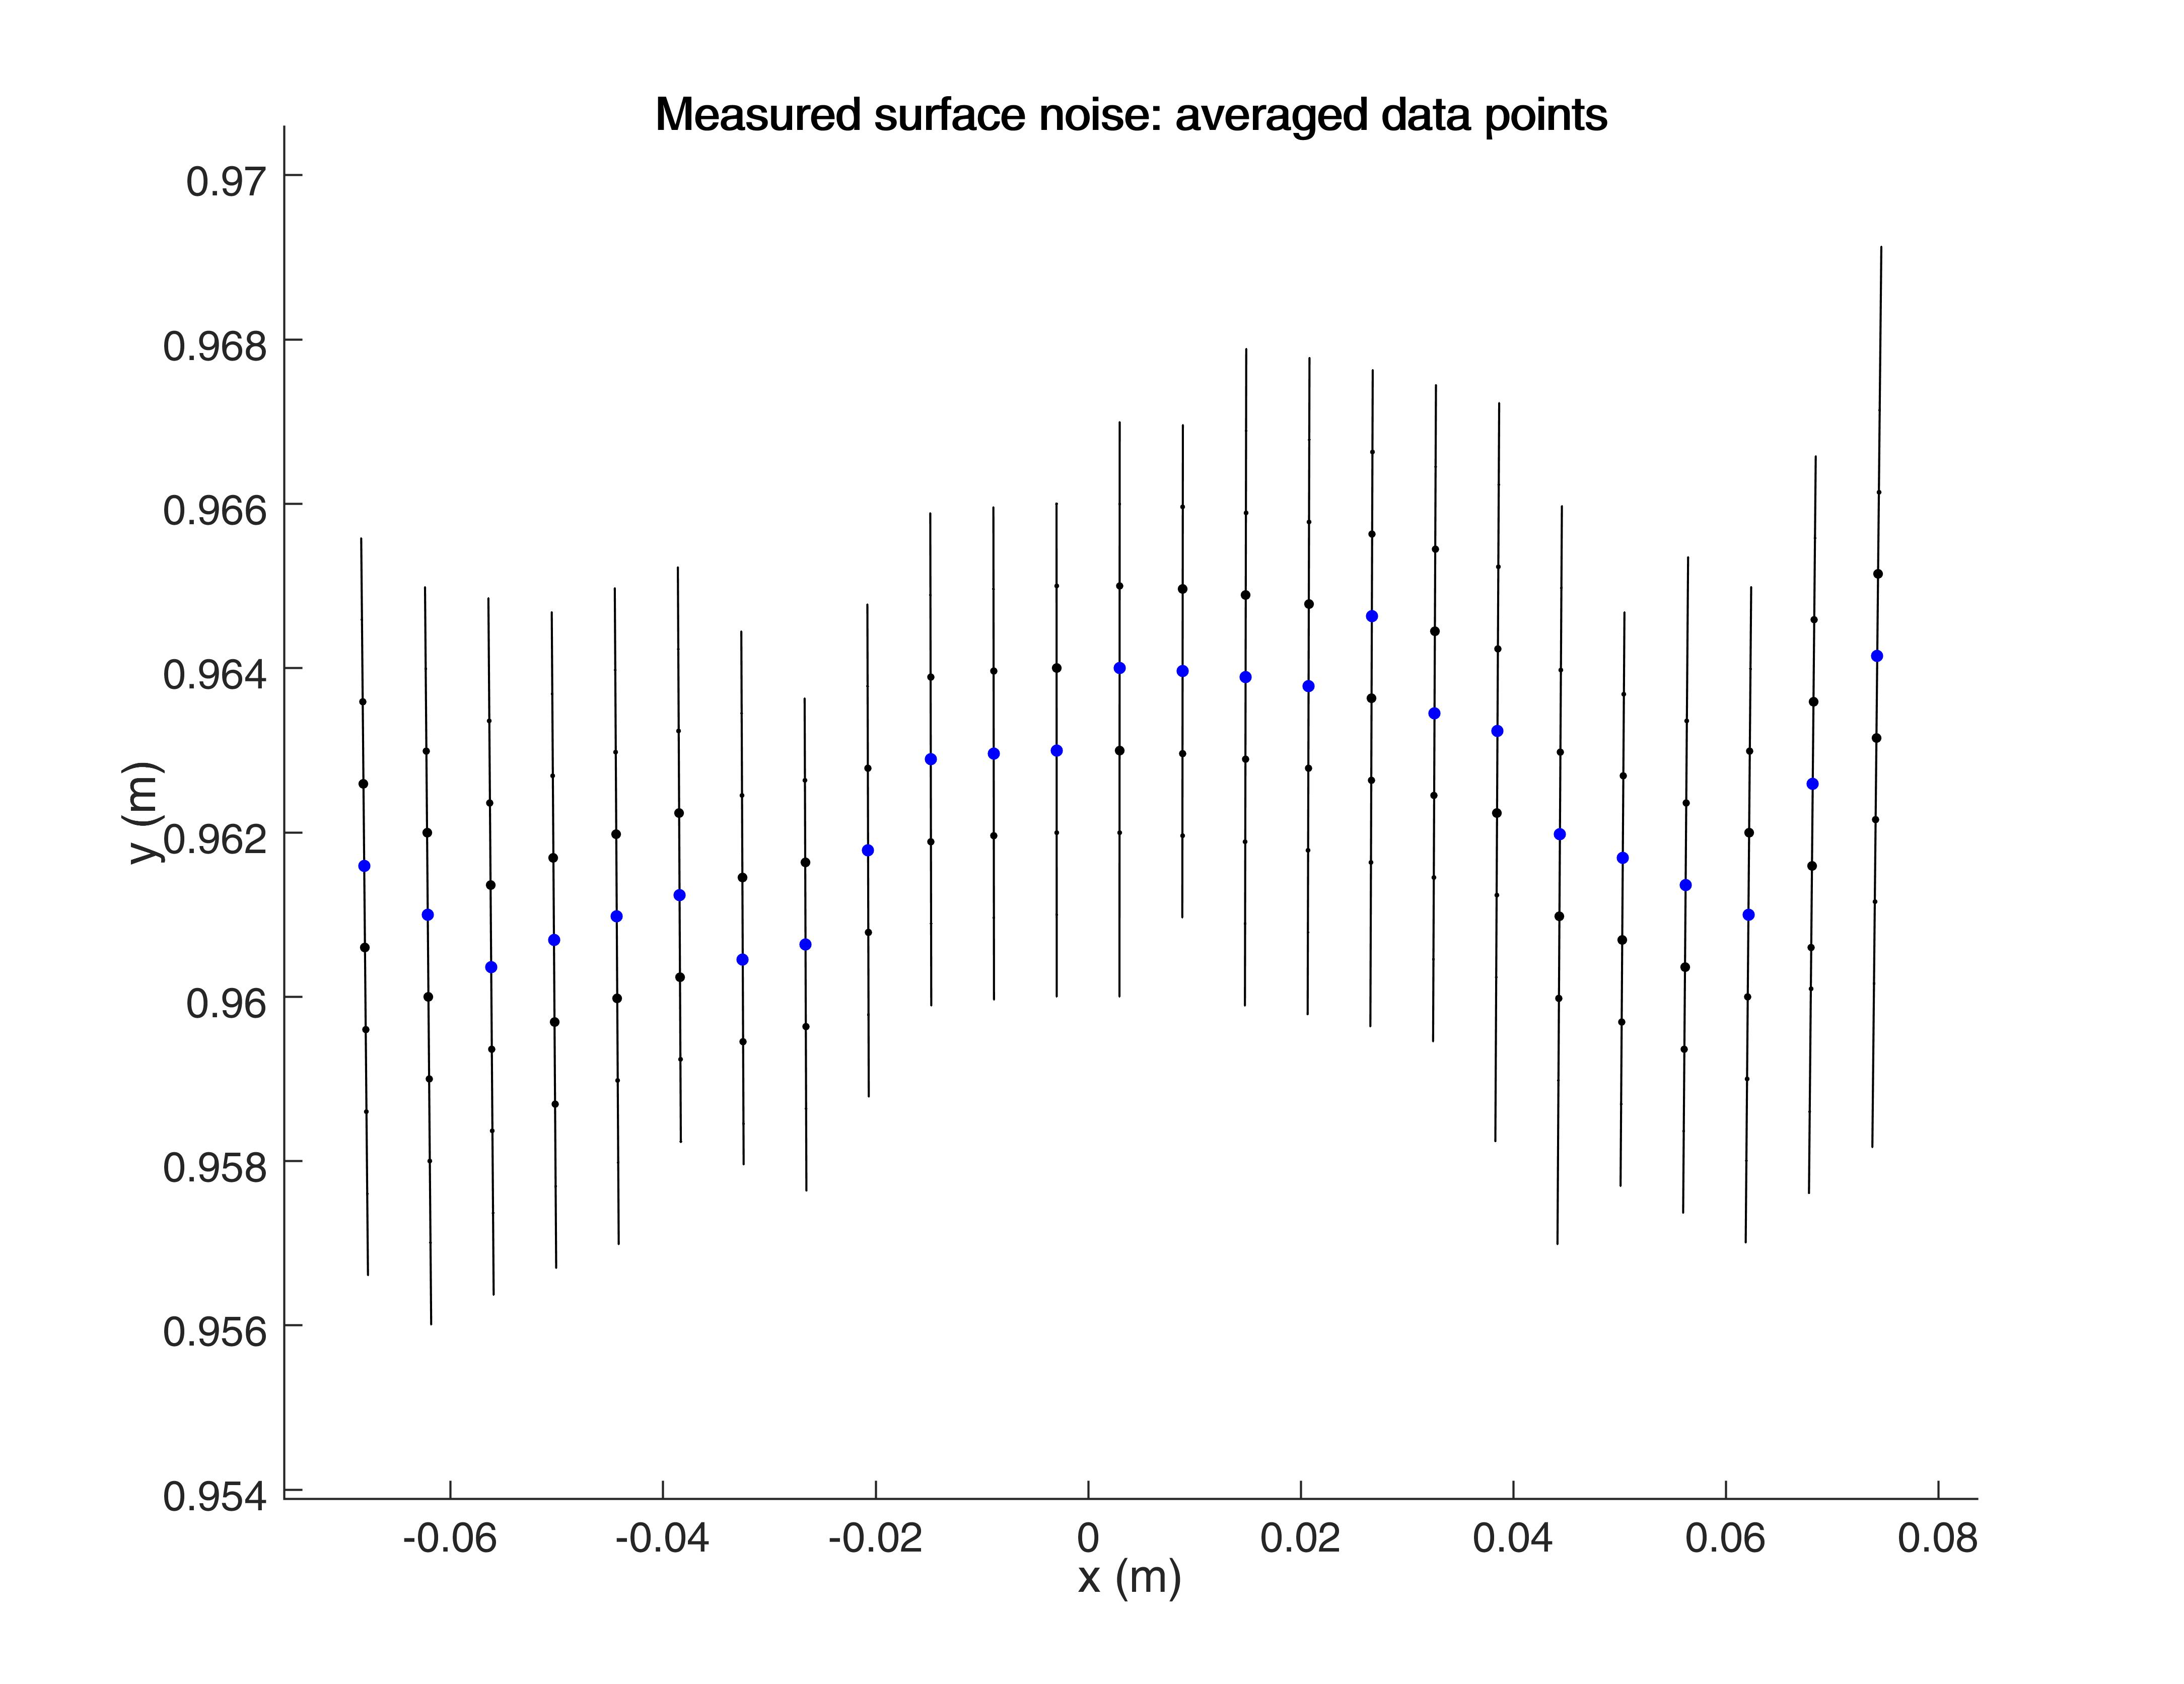
\includegraphics[width=1\textwidth,trim = 0mm 0mm 0mm 0mm,clip]{./Figures/measured_surface_noise}\vspace*{0ex}
	  		\end{minipage}}
	  		\subfigure[\label{fig:simulated_surface_noise}]{
	  		\begin{minipage}[b]{0.45\columnwidth}
    			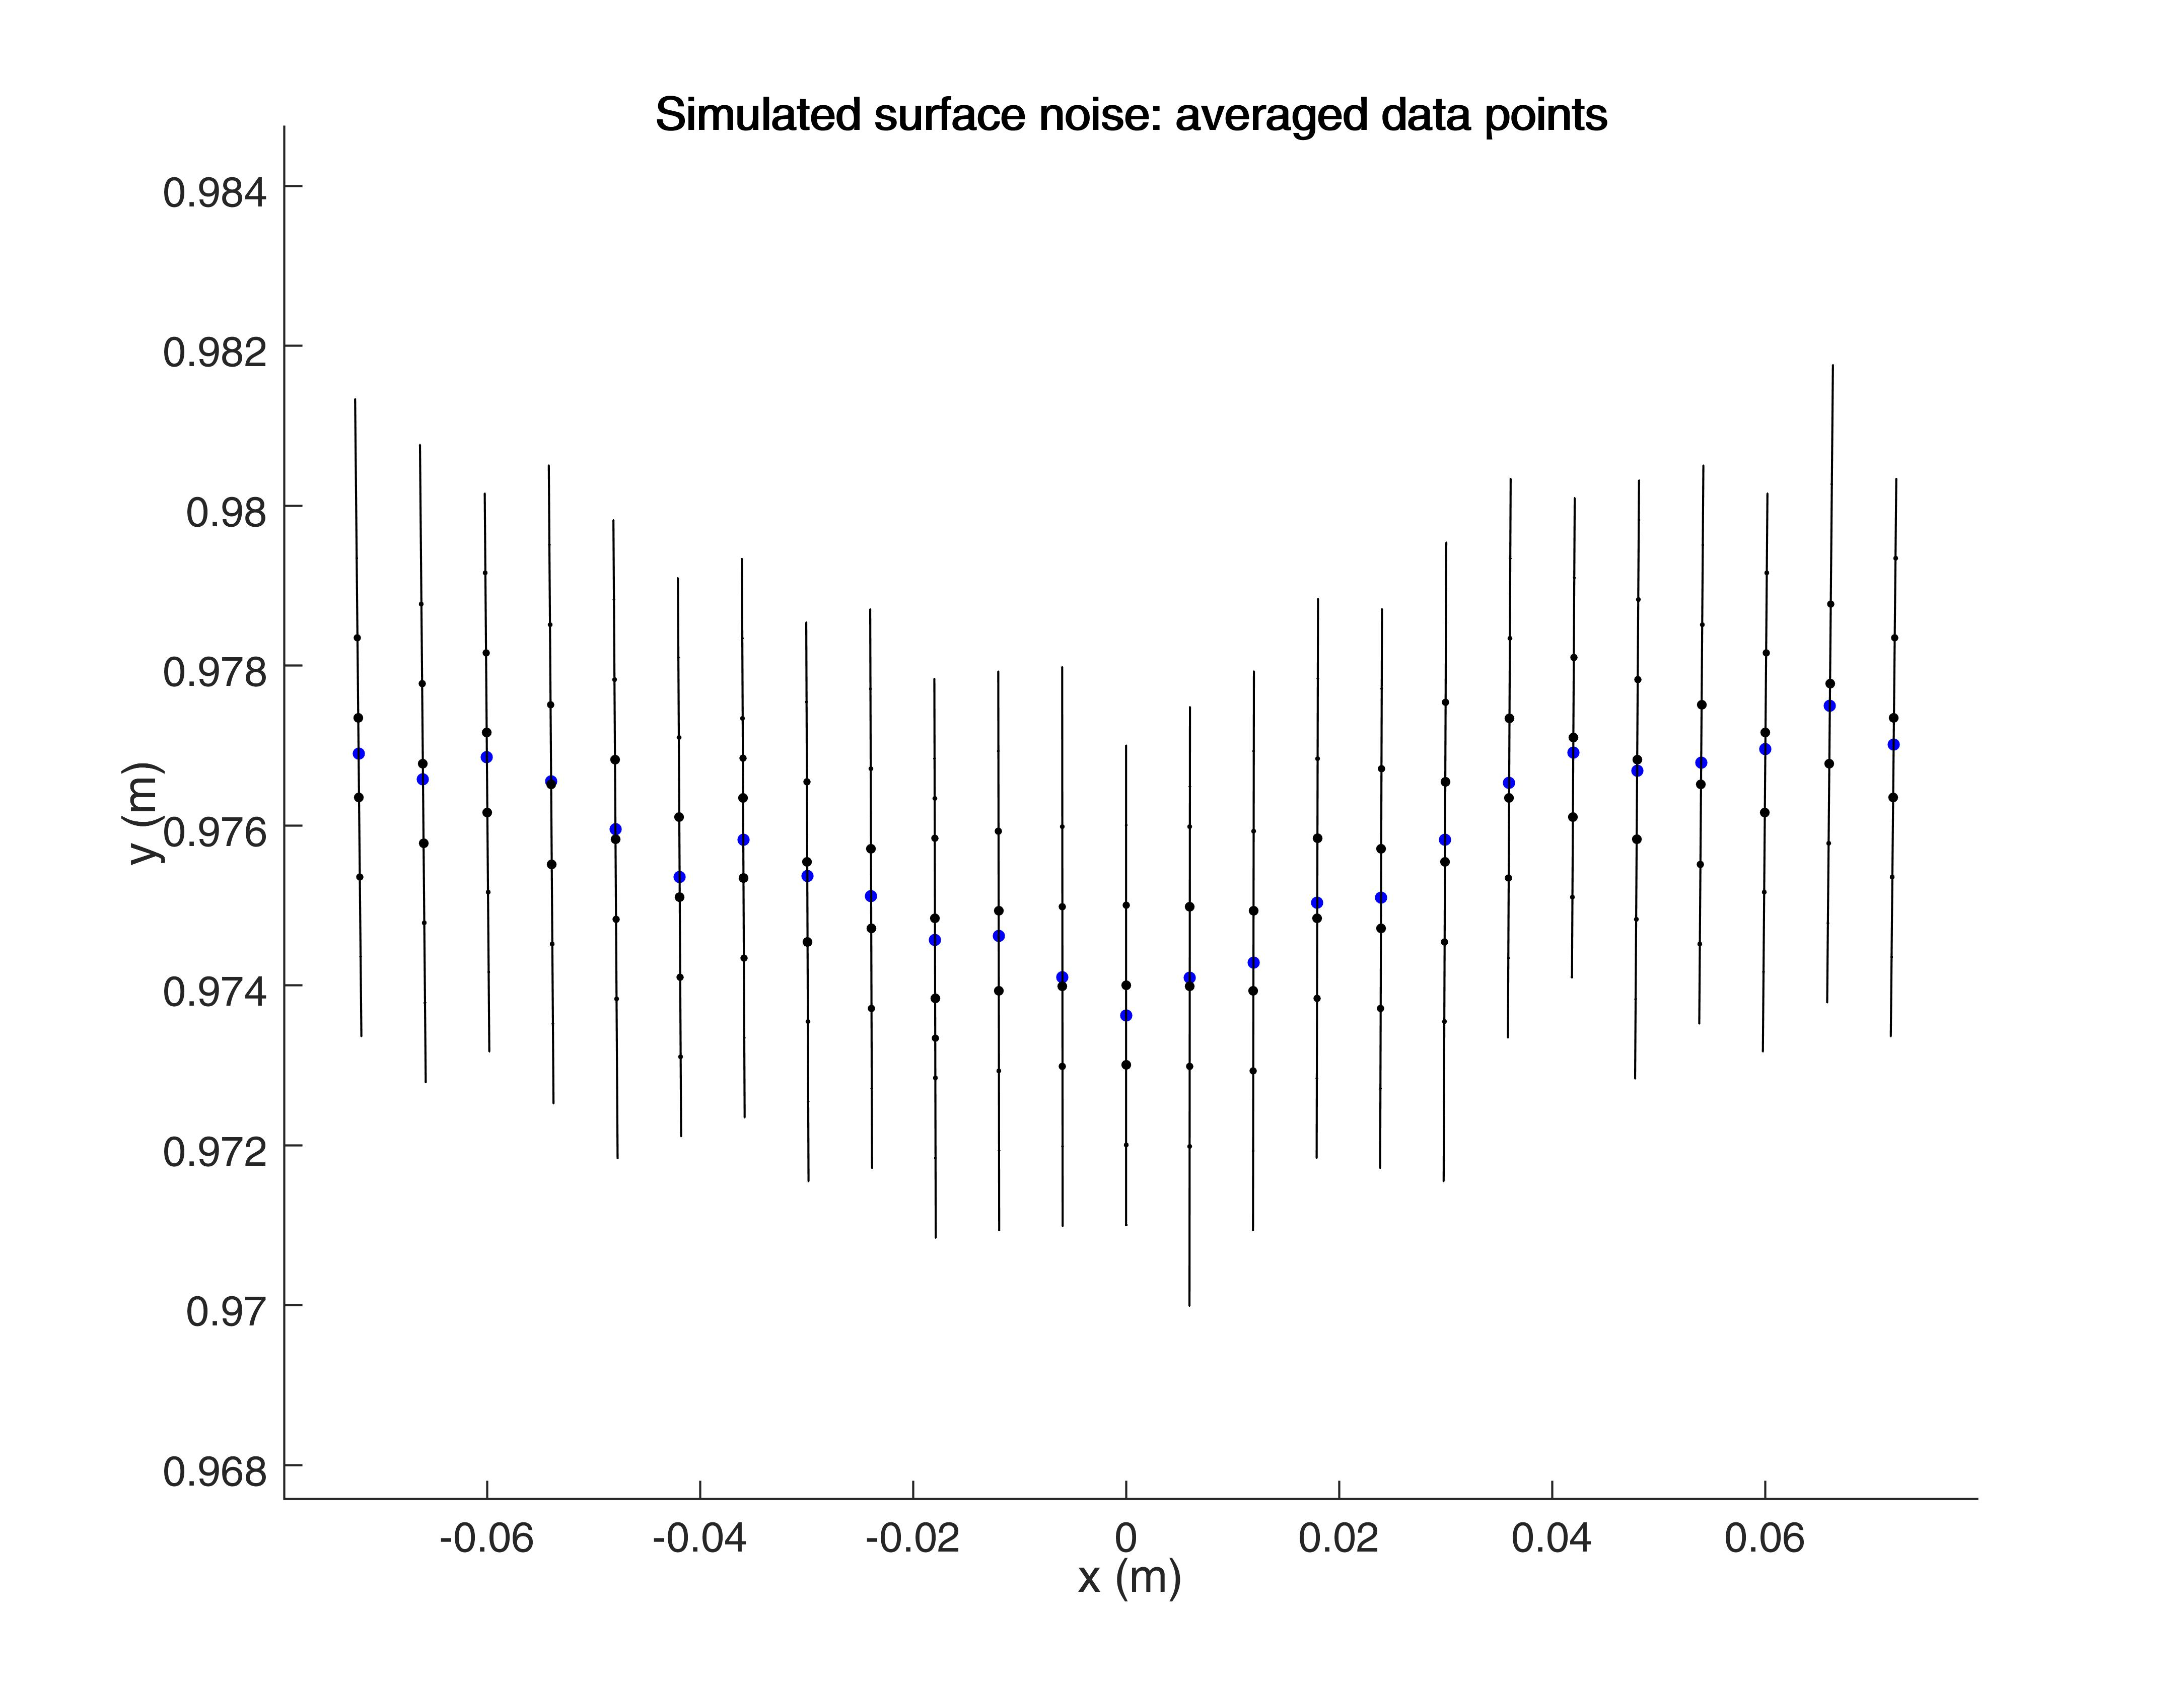
\includegraphics[width=1\textwidth,trim = 0mm 0mm 0mm 0mm,clip]{./Figures/simulated_surface_noise}\vspace*{0ex}
 			\end{minipage}}
	  		\caption{Comparision of (a) measured and (b) simulated surface noise. Point distribution along radial lines is shown as quintiles of error.}
	  		\label{fig:surface_noise}
		\end{figure}

\section{Observer Performance Testing Data} \label{testingdata}
	Data collected to assess the performance of the observer under real-world, less-than-ideal conditions.
	\subsection{Setup}
		The experimental setup is shown in Figure \ref{fig:experimental_data}.
		\begin{figure}
		\centering
			 	\includegraphics[width=0.75\textwidth,trim = 0mm 0mm 0mm 0mm,clip=true]{./Figures/experimental_data}\vspace*{0ex}
			  	\caption{setup to collect experimental data} \label{fig:experimental_data}
		\end{figure}

		The Hokuyo UBG-04LX-F01 sensor was mounted to a tripod. The sensor was panned up and down manually while the range and time recorded. This panning along with its own scanning behaviour allows the sensor to densely measure the infinite-dimensional environment depth field. To compute the elevation angle of the sensor, the range measurements to a portion of the blank wall were used. The range to this wall was measured at elevations increasing from  $-25^\circ$ to $25^\circ$ in $5^\circ$ increments for calibration purposes.
		
		The target object was a cube of 100mm side length cube made from medium-density fibreboard. The cube was spray painted matte white - the same surface as used in the sensor noise modelling in Section \ref{sensor_noise}.
		
		The cube was placed in the gripper of a Kinova Jaco robotic arm. The arm was manually manipulated to produce stationary, rotating, translating and combined motions. The joint angles of the sensor over time were recorded. From this data, the forward kinematic model for the arm was used to compute the ground truth pose of the cube over time.		
		
	\subsection{Results}
		Calibration of the data to determine the elevation angle of the sensor is yet to be completed. However, it is unlikely that the current implementation of the observer will be able to estimate the cube state from this data. Because the cube is held by the gripper of the arm, neither the range or continuity assumptions in Section \ref{separation} hold.  
		
		An infinite-dimensional observer measuring the entire depth field would give a better estimate of the state of the cube. A symmetry-preserving observer would likely be more robust to the significant levels of noise in the data set.


